\documentclass[review,3p]{elsarticle}

\usepackage{../../3_1d_or_2d/style_latex_custom}
\newcommand{\textif}[1]{\textbf{\textit{#1}}}

\newcommand{\cmark}{\ding{51}}%
\newcommand{\xmark}{\ding{55}}

\usepackage{tikzsymbols}

\usepackage{csquotes}
\usepackage{diagbox}
%\usepackage{slashbox}

\usepackage{amsmath}


\begin{document}

\begin{frontmatter}

\title{Balancing truncation and round-off errors in FEM: two-dimensional analysis}

\begin{abstract}
The round-off error is investigated when solving a problem using 2D FEM methods. We consider multiple FEM packages and multiple FEM methods. Different implementation gives different highest achievable accuracy. The round-off error can be well represented by the number of degrees of freedom (DoFs) and a coefficient related to the computer precision. 
The strategy in \cite{liu386balancing} for predicting the highest achievable accuracy is extended to 2D cases. The bound of the round-off error is determined by solving a problem with a manufactured solution. Using our strategy the time for obtaining the highest achievable accuracy can be saved ?\%.
\end{abstract}

\begin{keyword}
Finite Element Method, Round-off Error, 2D, Accuracy, Efficacy.
\end{keyword}

\end{frontmatter}

\section{Introduction}

In \cite{liu386balancing}, we observe the round-off error of one-dimensional second-order differential equations has a power-law relation with the number of DoFs, and the coefficient is relatively fixed. Based on that, we furthermore propose a strategy to predict the highest achievable accuracy. The algorithm for realising the strategy allows us to obtain the highest achievable accuracy correctly with a relatively small amount of CPU time. However, the study focuses on one-dimensional cases, and hence there is a lack of the analysis on two-dimensional cases, which is more and more widely used for practical problems. Therefore, the aim of the paper is to investigate the round-off error when solving 2D problems using FEM methods, and extend the strategy in \cite{liu386balancing} to 2D cases.

The 2D numerical analysis allows the solution to vary both in $x$ and $y$ directions, and hence the physical properties are better retained. In comparison with 1D problems, 2D problems have the following features. 
First, the problem size of 2D problems increases greatly. For example, using the standard FEM with the grid size $h$ and element degree $p$, the number of DoFs of 2D problems is the square of that of 1D problems. This increase inevitably entails much more CPU time and hence highlights the importance of the efficacy in solving the problem. Second, the derivatives of 2D problems are more complicated. One is that they contain more components than 1D problems do: the number of components for the first and second derivatives are 2 and 4, respectively, for 2D problems, but 1 for 1D problems; the other is that they have more types: they contain not only pure second derivatives, i.e. $u_{xx}$ and $u_{yy}$, but also mixed ones, i.e. $u_{xy}$ and $u_{yx}$, where $u$ is the unknown variable.

The round-off error is deeply related to the limitation in the capability of the IEEE (double) floating-point arithmetic, of which the precision is as high as $1 \times 10^{-16}$. Since this arithmetic is a common standard for scientific computing, we may observe its influence on the round-off error in different FEM packages and FEM methods. Therefore, here we investigate two FEM packages: one is deal.\rom{2}~\cite{bangerth2007deal}, the other one is FEniCS~\cite{alnaes2015fenics}. The former is written in C++ and constructed by quadrilaterals, and the latter is written in Python and constructed by triangles. Different grid types indicate different distributions of degrees of freedom and hence different ways of counting them.
In \cite{liu386balancing}, we find the mixed FEM produces higher accuracy than the standard FEM when the number of DoFs is relatively large, using the same element degree; this holds for both the solution and its first and second derivatives. We will demonstrate this for 2D problems using the above two packages.

The paper is organized as follows. The model problem, finite element formulation and numerical implementation are described in Section \ref{section_model_problem_FEM_formulation_numerical_implementation}. The approach to predicting the highest achievable accuracy ${E}_{\rm {min}}$ is illustrated in Section \ref{section_error_evolution_and_prediction}. The study on the property of the round-off error is given in Section \ref{section_benchmark_problems}. The algorithm for realizing the approach is put forward in Section \ref{section_algorithm}, followed by its validation by a Helmholtz problem in Section \ref{section_validation}. The conclusions are drawn in Section \ref{paragraph_on_conclusion}.

\section{Model problem, finite element formulation and numerical implementation}	\label{section_model_problem_FEM_formulation_numerical_implementation}

\subsection{Model problem}				\label{section_model_problem}

We consider the following two-dimensional second-order differential equation:
\begin{equation}
 -\nabla \cdot \left(D(\mathbf{x}) \nabla u \right) + r(\mathbf{x})u(\mathbf{x}) = f(\mathbf{x}),\qquad \mathbf{x} \in \Omega = [0,\,1] \times [0,\,1],	\label{2d_second_order_differential_equation}
\end{equation}
where $u$ denotes the unknown variable, $f(\mathbf{x}) \in L_2 (\Omega)$ the prescribed right-hand side, and $D(\mathbf{x})$ and $r(\mathbf{x})$ the coefficient functions. $D(\mathbf{x})$ is assumed to be positive definite.
By choosing $D(\mathbf{x})$ as the identity matrix $I$ and $r(\mathbf{x})=0$, Eq.~(\ref{2d_second_order_differential_equation}) reduces to the Poisson equation; for $|D(\mathbf{x})|>$0, the diffusion equation is found when $r(\mathbf{x})=0$, and the Helmholtz equation is found for $r(\mathbf{x}) \neq $ 0. 
The boundary conditions are $u(\mathbf{x})=g(\mathbf{x})$ on $\Gamma_D$ and $D(\mathbf{x})\nabla u=\mathbf{h}(\mathbf{x})$ on $\Gamma_N$. Here, $\Gamma_D$ and $\Gamma_N$ are the boundaries where Dirichlet boundary conditions and Neumann boundary conditions are imposed, respectively. It is important to note that we assume the second derivative exists in the weak sense, i.e. $u \in H^2(\Omega)$ for Eq.~(\ref{2d_second_order_differential_equation}), even though this is only guaranteed for Poisson equations~\cite[p.~9]{boffi2013mixed}.

\subsection{Finite element formulation} 	\label{FE formulation}
\subsubsection{Preliminaries}
\begin{subequations}
Before deriving the weak formulations, we define the following function spaces for a scalar function $t(x,y)$~\cite{quoraSCALARfunction}. First, the space of square integrable functions on $\Omega$~\cite{boffi2013mixed}:
\begin{align}
  L_2(\Omega) := \bigg\{ t \Big| \int_{\Omega} | t |^2 dx = \| t \|_{L_2(\Omega)} ^2 < +\infty \bigg\}.   \label{definition_l2_space}
\end{align}
Second, a general form of Eq.~(\ref{definition_l2_space}) that concerns not only the variable $t$ itself but also its derivatives~\cite{boffi2013mixed}:
\begin{align}
  H^m(\Omega):= \bigg\{ t \Big| D^{\alpha}t \in L_2(\Omega),  \qquad \forall |\alpha| \leq m \bigg\},	\label{definition_hm_space}
\end{align}
where $m \geq 0$ and
\begin{align*}
  D^{\alpha}t := \frac{\partial ^{|\alpha|}t}{\partial x ^{\alpha_1} \partial y ^{\alpha_2}} \qquad |\alpha| = \alpha_1 + \alpha_2.
\end{align*}
Obviously, higher-order derivatives are concerned with increasing $m$. Specifically,
\begin{align*}
  H^0(\Omega) &:= L_2(\Omega), \\
  H^1(\Omega) &:= \bigg\{ t \in L_2(\Omega) \Big| \frac{\partial t}{\partial x}, \frac{\partial t}{\partial y} \in L_2(\Omega) \bigg\}, \text{ and } \\
  H^2 (\Omega) &:= \bigg\{ t \in H^1(\Omega) \Big| \frac{\partial ^2 t}{\partial ^2 x}, \frac{\partial ^2 t}{\partial y ^2},\frac{\partial ^2 t}{\partial x \partial y} \in L_2(\Omega) \bigg\}
\end{align*}
\end{subequations}
For a vector function $\mathbf{t}(x,y)$~\cite{quoraSCALARfunction}, we define the following function spaces~\cite{rognes2010efficient}:
\begin{align}
  H(div,\Omega) := \bigg\{ \mathbf{t} \in L_2(\Omega,\mathbb{R}^2) \Big| \nabla \cdot \mathbf{t} \in L_2(\Omega)  \bigg\}.
\end{align}

\begin{subequations}
For convenience, we introduce three inner products~\cite{lipschutz2009linear}:
  \begin{align}
   \langle \mathbf{f}_1, \,\mathbf{f}_2 \rangle &= \int _{\Omega} \mathbf{f}_1(\mathbf{x}) \cdot \mathbf{f}_2(\mathbf{x}) \, d A,	\\
   \langle f_1, \,f_2 \rangle &= \int _{\Omega} f_1(\mathbf{x}) f_2(\mathbf{x}) \, d A,	\text{ and}\\
   \langle f_1, \,f_2 \rangle _{\Gamma} &= \int _{\Gamma} f_1(\mathbf{x}) f_2(\mathbf{x}) ds,
  \end{align}
\end{subequations}
where $\mathbf{f}_1(\mathbf{x})$ and $\mathbf{f}_2(\mathbf{x})$ denote continuous vector-valued functions of length 2, and $f_1(\mathbf{x})$ and $f_2(\mathbf{x})$ denote continuous scalar functions. $\Gamma$ denotes the boundary of $\Omega$.



\subsubsection{The standard FEM}

The weak form of Eq. (\ref{2d_second_order_differential_equation}) is derived in \ref{derivation_weak_form_SM}. Imposing the Dirichlet boundary conditions strongly, the weak form reads~\cite{chen2005finite}:
\begin{equation}
\centering
\boxed{ 
\begin{aligned}
&\text{Weak~form}~ 1 ~~~~~~~~~\\
&\text{Find $u \in H _D^1 (\Omega)$ such that:} \\
& \langle {\nabla \eta}, \, D \nabla u \rangle + \langle \eta, \, ru \rangle = \langle \eta, \, f \rangle + \langle \eta, \, \mathbf{h} \cdot \mathbf{n} \rangle_{ {\Gamma_N}}. \qquad \forall \eta \in H _{D0}^1 (\Omega),\\
&\text{with} \\
&~~~~~~~~~~~~~H_{D} ^1 (\Omega) = \{t \; | \; t \in H^1 (\Omega), \; t = g \text{ on } \Gamma _D \},  \\
&~~~~~~~~~~~~H_{D0} ^1 (\Omega) = \{t \; | \; t \in H^1 (\Omega), \; t = 0 \text{ on } \Gamma _D\}.\\
\end{aligned}		\label{sm_weak_form_Diri_strong} 
}
\end{equation}

\noindent$\eta$ denotes the test function, $\mathbf{n}$ is the unit normal vector; the terms in the right-hand sides consist of information of Neumann boundary conditions which vanishes if no Neumann boundary conditions are prescribed. We approximate $u$ by a linear combination of a finite number of basis functions:
\begin{equation}
 u \approx u_h ^{(p)} = \sum _ {i=1} ^{m} u _{i} \varphi _{i}^{(p)}. \label{sm_u_approx}%
\end{equation}
Here, $p$ is the element degree, $m$ is the number of DoFs over the whole domain, which equals $(p \times 2^R + 1)^2$, where $R$ denotes the number of refinements; $u_i$'s are the values of $u_h^{(p)}$ at the DoFs; $\varphi _{i}^{(p)}$'s are $C^0$-continuous Lagrange basis functions supported by Gauss-Lobatto points, which feature the Kronecker-delta property, i.e. $\varphi _{i}^{(p)} (\mathbf{x}_j)=\delta_{ij}$, where $\mathbf{x}_j$ denotes the support point. This type of element will be referred to as $Q_p$.
Note that, the number of DoFs is counted based on problems with real-valued solution, and hence it doubles for problems with complex-valued solution.

Substituting the test functions, the resulting linear system of equations reads
\begin{equation}
 A {U} = F,				\label{matrix_equation_std}
\end{equation}
where $A$ is the stiffness matrix, $F$ the right-hand side and $U$ the numerical solution of $u$ at DoFs.

\subsubsection{The mixed FEM}
As a first step, we introduce the auxiliary variable
\begin{subequations}
\begin{align}
	\mathbf{v}(\mathbf{x}) = - D(\mathbf{x})\nabla u, \label{mm_strong_form_1} 
\end{align}  
allowing Eq. (\ref{2d_second_order_differential_equation}) to be rewritten as
\begin{align}
  -\nabla \cdot \mathbf{v} - r(\mathbf{x})u(\mathbf{x}) = -f(\mathbf{x}).  \label{mm_strong_form_2}
\end{align}	\label{mm_strong_form_block}%
\end{subequations}
The weak form of Eq. (\ref{2d_second_order_differential_equation}) using the mixed FEM, derived in \ref{derivation_weak_form_MM}, is given by:
\begin{subequations}
\begin{empheq}[box=\fbox]{align}
&\text{Weak~form}~ 2 ~~~~~~~~~\notag\\
&\text{Find $\mathbf{v} \in H_{N} (div, \Omega)$ and $u \in L ^2 (\Omega)$ such that:}	\notag\\
& ~~~~~~~\;\langle \mathbf{w}, \, D^{-1} \mathbf{v} \rangle - \langle \nabla \cdot \mathbf{w}, \,  u \rangle = -\langle \mathbf{w} \cdot \mathbf{n}, \, g \rangle_{\Gamma_D} \qquad \forall w \in H_{N0} (div, \Omega), \label{mm_weak_form_1}\\ 
& ~~~~~~~~~- \langle q, \, \nabla \cdot \mathbf{v} \rangle - \langle q, \, ru \rangle = -\langle q, \, f \rangle \qquad \forall q \in L ^2 (\Omega), \label{mm_weak_form_2}	\\
&    \text{with}\notag\\
& ~~~~~~~~~~~~~~~ H_{N} (div, \Omega) = \{\mathbf{t} \; | \; \mathbf{t} \in H (div, \Omega), \; \mathbf{t} = -\mathbf{h} \text{ on } \Gamma _N \},  \notag\\
& ~~~~~~~~~~~~~\, H_{N0} (div, \Omega) = \{\mathbf{t} \; | \; \mathbf{t} \in H (div, \Omega), \; \mathbf{t} = 0 \text{ on } \Gamma _N\}.	\notag 
\end{empheq}
\label{mm_weak_form_block}%
\end{subequations}
In Eq.~(\ref{mm_weak_form_block}), $\mathbf{w}$ and $q$ denote the test functions of $\mathbf{v}$ and $u$, respectively, and $\mathbf{n}$ has the same interpretation as before. 
\begin{subequations}
If the auxiliary variable is taken to be the opposite of the gradient of the solution, i.e.
\begin{align}
 \mathbf{v}(\mathbf{x}) = - \nabla u, 			  \label{mm_alter_strong_form_1}
\end{align}
which is utilized in calculating the advection term in \cite{kumar2017three}, then Eq.~(\ref{2d_second_order_differential_equation}) can be rewritten as
\begin{align}
 -\nabla \cdot (D(\mathbf{x}) \mathbf{v(\mathbf{x})}) - r(\mathbf{x})u(\mathbf{x}) = -f(\mathbf{x}).  \label{mm_alter_strong_form_2}
\end{align}
\end{subequations}

Using the above representations, the weak form, of which the derivation process is similar to Eq.~(\ref{mm_weak_form_block}), reads:
\begin{subequations}
\begin{empheq}[box=\fbox]{align}
&\text{Weak~form}~ 3 ~~~~~~~~~\notag\\
&\text{Find $\mathbf{v} \in H_{N} (div, \Omega)$ and $u \in L ^2 (\Omega)$ such that:}	\notag\\
& ~~~~~~~\;\langle \mathbf{w}, \, \mathbf{v} \rangle - \langle \nabla \cdot \mathbf{w}, \,  u \rangle = -\langle \mathbf{w} \cdot \mathbf{n}, \, g \rangle_{\Gamma_D} \qquad \forall w \in H_{N0} (div, \Omega), \label{mm_alter_weak_form_1}\\ 
& ~~~~~~~~~- \langle q, \, \nabla \cdot (D\mathbf{v}) \rangle - \langle q, \, ru \rangle = -\langle q, \, f \rangle \qquad \forall q \in L ^2 (\Omega), \label{mm_alter_weak_form_2}	\\
&    \text{with}\notag\\
& ~~~~~~~~~~~~~~~ H_{N} (div, \Omega) = \{\mathbf{t} \; | \; \mathbf{t} \in H (div, \Omega), \; \mathbf{t} = - D^{-1} \mathbf{h} \text{ on } \Gamma _N \},  \notag\\
& ~~~~~~~~~~~~~\, H_{N0} (div, \Omega) = \{\mathbf{t} \; | \; \mathbf{t} \in H (div, \Omega), \; \mathbf{t} = 0 \text{ on } \Gamma _N\}.	\notag 
\end{empheq}
\label{mm_alter_weak_form_block}%
\end{subequations}
$\mathbf{w}$, $q$ and $\mathbf{n}$ have the same meaning as before. We use Eq.~(\ref{mm_weak_form_block}) if not stated otherwise.

One feature of the 2D mixed FEM is the adoption of non-primitive finite elements for the auxiliary variable~\cite{dealiiRTelement}. Here, we implement the widely used Raviart-Thomas elements ($RT_p$) and Brezzi-Douglas-Marini elements ($BDM_p$)~\cite{rognes2010efficient}, where $p$ still denotes the element degree. The associated elements for $u$ are discontinuous Lagrangian polynomials of degree $p$ ($Q_p^{\rm disc}$) for the former and discontinuous Legendre elements of degree $p-1$ ($P_{p-1}^{\rm disc}$) for the latter, where `disc' denotes the elements for $u$ are discontinuous. The property of these element pairs is introduced below.

\paragraph{\texorpdfstring{$RT_p/Q_{p}^{\rm disc}$}{RTpQpdisc} elemensts}
The distribution of degrees of freedom of $RT_p$ elements is referred to \cite[Chapter~2]{boffi2013mixed}: the number of DoFs is $p+1$ on an edge and $2 \times p \times (p+1)$ on a quad, resulting that the number of DoFs per cell is $2 \times (p+1) \times (p+2)$. $Q_p^{\rm disc}$ elements have the same property as $Q_p$ elements introduced for the standard FEM, except that there are two independent sets of DoFs along the cell interface. Obviously, the number of DoFs per cell is $(p+1)^2$ for $Q_p^{\rm disc}$ elements. 

\begin{subequations}
Countably, for a unit square refined $R$ times, the number of DoFs for $\mathbf{v}$ reads
\begin{align}
 N_{\mathbf{v}} = \underbrace{(2^R +1) \times 2}_{A_1} \times \underbrace{(p+1) \times 2^R}_{A_2} +\underbrace{4^R}_{B_1} \times \underbrace{2 \times p \times (p+1)}_{B_2},
\end{align}
where $A_1$ denotes the number of longest edges, of which the grid size is 1, on the domain, $A_2$ denotes the number of DoFs on a longest edge, $B_1$ denotes the total number of smallest cells, and $B_2$ denotes the number of DoFs inside a smallest cell; the number of DoFs for $u$ reads
\begin{align}
 N_u = 4^R \times (p+1)^2.
\end{align}
\end{subequations}

Since the composition of $RT_p$ elements is relatively complicated~\cite{dealiiRTelement}, we do not illustrate the explicit approximation of $\mathbf{v}$ here, and refer to Eq.~(\ref{mm_rt_u_approx}) for the approximation of $u$:
\begin{subequations}
 \begin{align}
 \mathbf{v} \approx \mathbf{v} _h^{(p)} &= ?,     \label{mm_rt_v_approx}  \\[3ex]
 u \approx u _h^{(p)} &= \sum\limits _ {j=1} ^{(p+1)^2} u _{sj} \psi _{j}^{(p)} \text{ in cell }s, \text{ for } s=1,\,2, \, \ldots, \,t, \label{mm_rt_u_approx}
\end{align}	\label{mm_rt_var_approx_block}%
\end{subequations}
where $t$ denotes the total number of cells, $u_{sj}$'s are values of $u_h^{(p)}$ at the DoFs, and $\psi _{j}^{(p)}$'s are discontinuous Lagrange polynomials.


\paragraph{\texorpdfstring{$BDM_p/P_{p-1}^{\rm disc}$}{BDMpPp-1disc} elemensts}
We also refer to \cite[Chapter~2]{boffi2013mixed} for the distribution of DoFs of $BDM_p$ elements: the number of DoFs on an edge is the same with that of $RT_p$ elements, but the number of DoFs on a quad is $p \times (p-1)$ instead, resulting that the number of DoFs per cell is $(p+1) \times (p+2)+2$. Legendre polynomials used here are $L_2$-orthogonal and normalized on the reference cell, resulting that the mass matrix is diagonal~\cite{dealiiDGPelement}.
The number of DoFs per cell is $p \times (p+1)/2$ for $u$~\cite{dealiiDGPelement}. Note that, the element degree for $u$ is one order lower than that for $\mathbf{v}$.

For a unit square refined $R$ times, the number of DoFs for $\mathbf{v}$ reads
\begin{subequations}
\begin{align}
 N_{\mathbf{v}} = \underbrace{(2^R +1) \times 2}_{A_1} \times \underbrace{(p+1) \times 2^R}_{A_2} + \underbrace{4^R}_{B_1} \times \underbrace{p \times (p-1)}_{B_3},
\end{align}
where $B_3$ denotes the number of DoFs inside a cell for $BDM_{p}$ elements; the number of DoFs for $u$ reads
\begin{align}
 N_u = 4^R \times \frac{p \times (p+1)}{2}.
\end{align}
\end{subequations}

The approximation of $\mathbf{v}$ is not shown for the same reason as $RT_{p}$ elements, and the approximation of $u$ will be added later.

Substituting the test functions, the resulting coupled linear system of equations that has to be solved reads:
\begin{equation}
 \left[ \begin{array}{cc} M & B  \\ B^\top & W \end{array}\right] \left[ \begin{array}{cc} {V} \\ {U} \end{array}\right] =\left[ \begin{array}{cc} G \\ H \end{array}\right], \label{matrix_equation_mix}
\end{equation}
where the mass matrix $M$ on $H(div, \Omega)$, discrete gradient operator $B$, its transpose, which is the discrete divergence operator $B^\top$, and the mass matrix $W$ on $L_2(\Omega)$, comprise the left-hand side; $G$ and $H$ are the components of the right-hand side. $V$ and $U$ denote the numerical solution of $\mathbf{v}$ and $u$ at DoFs.

\subsection{Numerical implementation}					\label{numerical_implementation}

\subsubsection{Solution technique}

All results are computed in IEEE-754 double precision \cite{zuras2008ieee} using the deal.\rom{2} finite element library \cite{bangerth2007deal}. Unless stated otherwise, the computational mesh is obtained by globally refining a single element that covers the unit square $\Omega$, and the Dirichlet boundary conditions are imposed strongly. Since deal.\rom{2} does not provide native support for complex-valued problems, and hence all components need to be split into their real and imaginary parts.

To compute the occurring integrals, sufficiently accurate Gaussian quadrature formulas are used. 
To solve the systems of equations, the UMFPACK solver \cite{davis2004algorithm}, which implements the multi-frontal LU factorization approach, is used unless stated otherwise. This solver results in relatively fast computations of the problems considered in this paper, and prevents the iteration errors of iterative solvers. The derivatives of the numerical solution are computed in the classical finite element manner, e.g. $u_{h,x}=\sum\limits _{i=1}^m u_i\varphi_{i,x}$ yields an approximation to $u_x$ using standard FEM.
%\newpage
\subsubsection{Error estimation}

We measure the error of a variable ($var$) in the function space that defines it, which basically involves the $L_2$ norm~\cite{ref1} only. The error is defined as
\begin{equation}
 E_{h} = {\|var_{h}- \hat{var} \|_{2}},			\label{formular_error_l2}
\end{equation}
where $var_h$ denotes the numerical solution of grid size $h$, and $\hat{var}$ denotes the reference solution.
The latter is the exact solution when the exact solution is available and the solution of grid size $h/2$ otherwise~\cite{Runborg2012VerifyingNC}.

The variable $var$ may contain only one component such as $u$ for both the standard FEM and the mixed FEM, or multiple components, such as $\nabla u$ in the standard FEM and $\mathbf{v}$ in the mixed FEM. For the latter, Eq.~(\ref{formular_error_l2}) can be further written as~\cite{bangerth2007deal,boffi2013mixed}
\begin{equation}
 E_{h} = \sqrt{\sum _{i=1} ^{n_c} (\|var_{h}(i)- \hat{var}(i)\|_{2})^2},			\label{formular_error_l2_vector}
\end{equation}
where $n_c$ denotes the number of components in a variable.
That is, we compute the $L_2$ error of each variable component and then obtain the square root of the sum of their squares.

With respect to the numerical solution, since $u \in H^1(\Omega)$ for the standard FEM, and $u \in L_2(\Omega)$ and $\mathbf{v} \in H(div,\Omega)$ for the mixed FEM, the quantities which can be evaluated using Eq.~(\ref{formular_error_l2}) are up to $\nabla u = [ u_x,u_y ]^{\top}$ using the standard FEM, and up to $\nabla \cdot \mathbf{v} = [\partial / \partial x, \partial / \partial y]^{\top} \cdot [v_1, v_2]^{\top} = v_{1x} + v_{2y}$ using the mixed FEM. Note that, $\nabla \cdot \mathbf{v}$ only consists of pure second derivatives, i.e. $u_{xx}$ and $u_{yy}$, when $\mathbf{v} = -\nabla u$, and also consists of mixed second derivatives, i.e. $u_{xy}$ and $u_{yx}$, when $\mathbf{v} = -D(\mathbf{x}) \nabla u$ and $D(\mathbf{x})$ is not diagonal, using the mixed FEM.
A summary of the above quantities can be found in Table~\ref{components_existent_numerically}.
Note that, $\| \nabla u \|_2$ is also called the $H_1$ semi-norm of $u$, and $\| \nabla \cdot \mathbf{v} \|_2$ the $H(div,\Omega)$ semi-norm of $\mathbf{v}$~\cite{bangerth2007deal}.

\begin{table}[!ht]
\caption{Quantities of which the $L_2$ norm exists in theory.}
\label{components_existent_numerically}
\centering
\small
\begin{tabular}{c|c|c}
 Type of quantities & The standard FEM & The mixed FEM \\ \hline
 Solution & $u$ & $u$ \\ \cline{1-3}
 Gradient & $ \nabla u $ & $ \mathbf{v} $ \\ \cline{1-3}
 Hessian & -- & $\nabla \cdot \mathbf{v}$ \\ 
\end{tabular}
\end{table}

Consequently, using Eq.~({\ref{formular_error_l2}}), we can only compute the error for the quantities in Table~\ref{components_existent_numerically}. Nevertheless, we will compute the error for the second derivative using the standard FEM, as a comparison with its counterpart $\nabla \cdot \mathbf{v}$ using the mixed FEM. The quantity that we are interested is the hessian matrix of $u$, i.e.
\begin{equation*}
  \mathbf{H}u = \begin{bmatrix} u_{xx} & u_{xy} \\ u_{yx} & u_{yy} \end{bmatrix},
\end{equation*}
or $\Delta u = u_{xx}+u_{yy}$ when only pure second derivatives are involved. 
In order to consider the mixed second derivatives when $D(\mathbf{x})=1$ for the mixed FEM, we also investigate the gradient of each component of $\mathbf{v}$, i.e.
\begin{equation*}
  \nabla \mathbf{v} = 
  \begin{bmatrix}
    v_{1x} & v_{1y} \\
    v_{2x} & v_{2y}
  \end{bmatrix}.
\end{equation*}
Furthermore, we also investigate each component of the aforementioned $\mathbf{H}u$ and $\nabla \mathbf{v}$.
To summarize, the quantities of which the error is calculated are shown in Table~\ref{components_being_computded_for_the_error}.

\begin{table}[!ht]
\caption{Quantities of which the error is computed.}
\label{components_being_computded_for_the_error}
\centering
\small
\begin{tabular}{c|c|c}
 Type of quantities & The standard FEM & The mixed FEM \\ \hline
 Solution & $u$ & $u$ \\ \cline{1-3}
 Gradient & $ \nabla u $ & $ \mathbf{v} $ \\ \cline{1-3}
 Hessian & \fbox{\makecell{$\mathbf{H}u$, each component of $\mathbf{H}u$,\\ and $\Delta u$}} & \makecell{$\nabla \cdot \mathbf{v}$ \\ \fbox{$\nabla \mathbf{v}$ and each component of $\nabla \mathbf{v}$}} \\ 
\end{tabular}
\end{table}


\newpage
\subsubsection{Convergence of the solution}
When the number of DoFs is relatively large, but the round-off error does not exceed the truncation error, the error converges at a fixed rate, known as asymptotic convergence rate, of which the value is one order higher than the approximation order \cite{gockenbach2006understanding}. In practice, the convergence rate in the numerical experiments can be calculated from 
\begin{equation}
  Q=\log _2 \left( \frac{E_{h}}{E_{h/2}} \right).  \label{formula_order_of_convergence_analytical_solution}
\end{equation}

\section{Sketch of the strategy to predict the highest attainable accuracy}      \label{section_error_evolution_and_prediction}

A conceptual sketch of $E_h$ against the number of DoFs ($N_h$) in a log-log plot can be found in Fig.~\ref{error_evolution_one_p}, also see \cite{butcher2016numerical}.

\begin{figure}[!ht]
\centering
   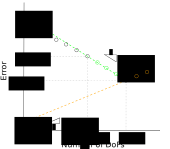
\includegraphics[width=0.5\linewidth]{../../3_1d_or_2d/3_figure/1_error_evolution_one_p/sketch_error_one_p.pdf}
   \caption{Conceptual sketch of the error evolution against the number of $\text{DoFs}$.}
   \label{error_evolution_one_p}
\end{figure}

When the number of DoFs is large enough, the error decreases at an asymptotic order with increasing number of DoFs.
The slope of the decreasing part of the error $\beta_{\rm T}$ is half of the asymptotic order of convergence for $u$ of the standard FEM and both $u$ and $\mathbf{v}$ of the mixed FEM, cf. \ref{proof_slope_ET}.

To determine the round-off error, we use the method of manufactured solutions~\cite{salari2000code,roache2002code,gfrerer2018code}. 

To make the method independent of $u$, we require $\|u\|_2$ is the same to that of the real problem.

Based on the round-off error, we determine the coefficients $\alpha_{R}$ and $\beta_{R}$ using the method of least squares.

\newpage
\section{2D problems}  	\label{section_benchmark_problems}

For the benchmark problems, we consider $u=(x-0.5)^2+(x-0.5)(y-0.5)+(y-0.5)^2$. The left and right boundaries are imposed by Dirichlet boundary conditions, and the upper and bottom boundaries are imposed by Neumann boundary conditions. Obviously, $u$ can be exactly approximated when the approximation order is larger than or equal to 2, and the first derivative can be exactly approximated when the approximation order is larger than or equal to 1.
We consider $D(\mathbf{x})$'s in Table~\ref{expression_coefficient_d}. 
They are all symmetric: $D(\mathbf{x})$ of Case 1 is an identity matrix, and that of Cases 2--3 varies; $D(\mathbf{x})$ of Case 3 cannot be represented exactly by (Lagrange) polynomials.
The property on the positiveness/definiteness can be found in the third column. 
The resulting $L_2$ norm of $\mathbf{v}$, denoted by $\| \mathbf{v} \|_2$, and right-hand side $f$ can be found in the last two columns.

\begin{table}[!ht]
\centering
\caption{Various $D(\mathbf{x})$'s.}
\small
\label{expression_coefficient_d}
  \begin{tabular}{c|c|c|c|c}
    Case & $D(\mathbf{x})$ & \makecell{Positiveness/ \\Definiteness} & $\| \mathbf{v} \|_2$ & $f$ \\ \hline
    1 & $I$& \multirow{2}{*}{Positive definite} &  &  \\ \cline{1-2} \cline{4-5}
    2 & $\big(\begin{smallmatrix} 1+x+y & xy \\ xy & 1+x+y \end{smallmatrix} \big)$ &  &  &  \\ \cline{1-5}
    3 & $\big(\begin{smallmatrix} e^{-[(x-0.5)^2+(y-0.5)^2]} & xy \\ xy & e^{-[(x-0.5)^2+(y-0.5)^2]} \end{smallmatrix} \big)$ & Indefinite as a whole & &  \\ 
  \end{tabular}
\end{table}

We are able to implement $Q_p$, $RT_p/Q_p^{\rm disc}$ and $BDM_p/P_{p-1}^{\rm disc}$ elements for all the cases, but all results are unavailable now, c.f. Table~\ref{FEM_methods_for_diffusion_varying} for an overview.

\begin{table}[!ht]
\caption{Current status of the results for the benchmark problems in Table~\ref{expression_coefficient_d}.}
\footnotesize
\centering
 \begin{tabular}{c|l|c|c|c}
\multicolumn{2}{c|}{Case} & 1 & 2 & 3 \\ \hline
\multirow{3}{*}{\makecell{Element type\\ in deal.\rom{2}}} & $Q_p$ & \xmark \footnotemark[1] & \xmark & \xmark \\ \cline{2-5}
& $RT_p/Q_p^{\rm disc}$& \xmark & \xmark & \xmark \\ \cline{2-5}
& $BDM_p/P_{p-1}^{\rm disc}$ & \xmark & \xmark & \xmark \\ 
\end{tabular}
\label{FEM_methods_for_diffusion_varying}
\end{table}

\footnotetext[1]{Results not available.}

%Using different finite elements, i.e. $Q_p$, $RT_p/Q_p^{\rm disc}$ and $BDM_p/P_{p-1}^{\rm disc}$, the error is shown in Figs.?. As can be seen, the round-off error increases along a straight line with the number of DoFs for all the FEM methods. 
%Interestingly, for the same number of DoFs, the round-off errors of different $p$'s are basically the same for $Q_p$ and $RT_p/Q_{p}^{\rm disc}$ elements; the round-off error of higher $p$ tends to be larger for $BDM_p/P_{p-1}^{\rm disc}$ elements.
%
%
%\paragraph{Case 1}
%%\newpage
%\paragraph{Case 2}
%%\newpage
%\paragraph{Case 3}

\newpage

\section{1D problems}					\label{section_decrease_beta_r_1d}

In this section, we investigate the decrease of the slope of the round-off error $\beta_{\rm R}$.
We consider 1D problems for which both boundaries are imposed by Dirichlet boundary conditions. 

For all the error plots, we use a straight line to approximate the round-off error.
To determine this line, we use the relatively larger round-off error, which occurs mostly when $p>2$.
The line color is red for the Poisson problems with the uniform mesh and orange otherwise because the round-off error of the latter might be smaller.
For the problems which are not the Poisson problem of the uniform mesh, we also plot the line of the round-off error for it, to have a comparison.

\subsection{Poisson problems}			\label{section_decrease_beta_r_1d_pois}

We investigate the Poisson problems in Table~\ref{results_various_Pois_1d_dealii}.
$u$ is in the $Q_p$ space (made of Lagrange polynomials of order up to p) when $u=(x-0.5)^2$ and not in $Q_p$ space when $u=e^{-(x-0.5)^2}$; $\|u\|_2$ of the second case (0.92) is about 10 times of that of the first case (0.11).
For each problem, we use four kinds of mesh: mesh without distortion, mesh distorted randomly, the first type of regularly distorted mesh and the second type of regularly distorted mesh, c.f. Section~\ref{section_poisson_mesh_distortion} for the settings of the distorted mesh.

A summary of the resulting $\beta_{\rm R}$ and $\alpha_{\rm R}$ can be found in Table~\ref{results_various_Pois_1d_dealii}, and an illustration of their contribution to the round-off error can be found in Fig.~\ref{alpha_R_beta_R_mesh_0_pois_0_u_x_m_0p5_square_0_sm} for $u=(x-0.5)^2$ and Fig.~\ref{alpha_R_beta_R_mesh_0_pois_1_u_exp_m_x_m_0p5_square_0_sm} for $u=e^{-(x-0.5)^2}$.
Based on both figures, the round-off error of the distorted mesh basically follows that of the uniform mesh, for which $\beta_{\rm R}$ is 2.0, and $\alpha_{\rm R}$ is basically proportional to $\|u\|_2$. 
We notice that when using the third type of mesh, i.e. the distorted mesh of Eq.~(\ref{regular_mesh_2}), the round-off error of $u$ and $u_x$ will become smaller: $\beta_{\rm R}$ decreases to 1.5, and $\alpha_{\rm R}$ basically does not change when $u=(x-0.5)^2$; $\beta_{\rm R}$ does not change, and $\alpha_{\rm R}$ decreases when $u=e^{-(x-0.5)^2}$.

\begin{table}[!ht]
\caption{Various Poisson problems and the resulting $\beta_{\rm R}$ and $\alpha_{\rm R}$ in deal.\rom{2}.}
\centering
\scriptsize
\begin{tabular}{l|c|c|c|c}
 \multirow{2}{*}{Distortion type} & \multicolumn{2}{c|}{$u=(x-0.5)^2$} & \multicolumn{2}{c}{$u=e^{-(x-0.5)^2}$} \\ \cline{2-5}
  & $\beta_{\rm R}$ & $\alpha_{\rm R}$ & $\beta_{\rm R}$ & $\alpha_{\rm R}$ \\ \hline
 Uniformly & 2.0 2.0 2.0 & 1e-18 5e-18 1e-16 & 2.0 2.0 2.0 & 2e-17 1e-16 5e-16 \\ \hline  
 Randomly & 2.0 2.0 2.0 & 1e-18 5e-18 2e-16 & 2.0 2.0 2.0 & 2e-17 1e-16 5e-15 \\ \hline
 Regularly of Eq.~(\ref{regular_mesh_1}) & 2.0 2.0 2.0 & 1e-18 5e-18 2e-16 & 2.0 2.0 2.0 & 2e-17 1e-16 2e-15 \\ \hline
 Regularly of Eq.~(\ref{regular_mesh_2}) & 1.5 1.5 2.0 & 2e-18 1e-17 1e-16 & 2.0 2.0 2.0 & 2e-18 5e-18 1e-15 \\ 
\end{tabular}
\label{results_various_Pois_1d_dealii}
\end{table}

\begin{figure}[!ht]
	\subfloat[$u$\label{alpha_R_beta_R_mesh_0_pois_0_u_x_m_0p5_square_0_sm_solu}]{\includegraphics[width=0.33\linewidth]{../2_figure/1_dealii/2_alpha_R_comparison/1d/0_pois/0_u_x_m_0p5_square/0_sm/py_alpha_R_beta_R_summary_mesh_1d_0_pois_0_u_x_m_0p5_square_0_sm_solu.pdf}}
    \subfloat[$u_x$\label{alpha_R_beta_R_mesh_0_pois_0_u_x_m_0p5_square_0_sm_grad}]{\includegraphics[width=0.33\linewidth]{../2_figure/1_dealii/2_alpha_R_comparison/1d/0_pois/0_u_x_m_0p5_square/0_sm/py_alpha_R_beta_R_summary_mesh_1d_0_pois_0_u_x_m_0p5_square_0_sm_grad.pdf}}
    \subfloat[$u_{xx}$\label{alpha_R_beta_R_mesh_0_pois_0_u_x_m_0p5_square_0_sm_2ndd}]{\includegraphics[width=0.33\linewidth]{../2_figure/1_dealii/2_alpha_R_comparison/1d/0_pois/0_u_x_m_0p5_square/0_sm/py_alpha_R_beta_R_summary_mesh_1d_0_pois_0_u_x_m_0p5_square_0_sm_2ndd.pdf}}
\caption{Illustration of $\beta_{\rm R}$ and $\alpha_{\rm R}$ using $Q_p$ elements for the 1D Poisson problem in deal.\rom{2}.}
\label{alpha_R_beta_R_mesh_0_pois_0_u_x_m_0p5_square_0_sm}
\end{figure}

\begin{figure}[!ht]
	\subfloat[$u$\label{alpha_R_beta_R_mesh_0_pois_1_u_exp_m_x_m_0p5_square_0_sm_solu}]{\includegraphics[width=0.33\linewidth]{../2_figure/1_dealii/2_alpha_R_comparison/1d/0_pois/1_u_exp_m_x_m_0p5_square/0_sm/py_alpha_R_beta_R_summary_mesh_1d_0_pois_1_u_exp_m_x_m_0p5_square_0_sm_solu.pdf}}
    \subfloat[$u_x$\label{alpha_R_beta_R_mesh_0_pois_1_u_exp_m_x_m_0p5_square_0_sm_grad}]{\includegraphics[width=0.33\linewidth]{../2_figure/1_dealii/2_alpha_R_comparison/1d/0_pois/1_u_exp_m_x_m_0p5_square/0_sm/py_alpha_R_beta_R_summary_mesh_1d_0_pois_1_u_exp_m_x_m_0p5_square_0_sm_grad.pdf}}
    \subfloat[$u_{xx}$\label{alpha_R_beta_R_mesh_0_pois_1_u_exp_m_x_m_0p5_square_0_sm_2ndd}]{\includegraphics[width=0.33\linewidth]{../2_figure/1_dealii/2_alpha_R_comparison/1d/0_pois/1_u_exp_m_x_m_0p5_square/0_sm/py_alpha_R_beta_R_summary_mesh_1d_0_pois_1_u_exp_m_x_m_0p5_square_0_sm_2ndd.pdf}}
\caption{Illustration of $\beta_{\rm R}$ and $\alpha_{\rm R}$ using $Q_p$ elements for the 1D Poisson problem in deal.\rom{2}.}
\label{alpha_R_beta_R_mesh_0_pois_1_u_exp_m_x_m_0p5_square_0_sm}
\end{figure}

\newpage
\subsection{Diffusion problems}			\label{section_decrease_beta_r_1d_diff}

We still investigate the same $u$'s but with various $D(\mathbf{x})$'s illustrated in Table~\ref{results_various_d_for_beta_r_decrease_1d_dealii}. When $D(\mathbf{x}) = 1+x$, we also use the regularly distorted mesh of Eq.~(\ref{regular_mesh_2}).
Using the uniform mesh, the error is shown in Fig.~\ref{py_1d_1_diff_0p00_u_x_m_0p5_square_d_1px_0_sm}--Fig.~\ref{py_1d_1_diff_0p4_u_x_m_0p5_square_d_exp_m_x_m_0p5_square_0_sm} when $u=(x-0.5)^2$ and Fig.~\ref{py_1d_1_diff_1p00_u_exp_m_x_m_0p5_square_d_1px_0_sm}--Fig.~\ref{py_1d_1_diff_1p2_u_exp_m_x_m_0p5_square_d_exp_m_x_m_0p5_square_0_sm} when $u=e^{-(x-0.5)^2}$.
For the distorted mesh, the error is shown in Fig.~\ref{py_1d_1_diff_0p01_u_x_m_0p5_square_d_1px_distorted_0_sm} and Fig.~\ref{py_1d_1_diff_1p01_u_exp_m_x_m_0p5_square_d_1px_distorted_0_sm}, respectively.

An overview of the resulting $\beta_{\rm R}$ and $\alpha_{\rm R}$ can be found in Table~\ref{results_various_d_for_beta_r_decrease_1d_dealii}, and their contribution to the round-off error can be found in Fig.~\ref{alpha_R_beta_R_mesh_1_diff_0_u_x_m_0p5_square_0_sm} and Fig.~\ref{alpha_R_beta_R_mesh_1_diff_1_u_exp_m_x_m_0p5_square_0_sm}, respectively, in which we also plot that of the Poisson problem.

From these figures, in comparison with the Poisson problem, the round-off error of $u_{xx}$ basically does not change, but that of $u$ and $u_x$ basically decreases. 
We describe the round-off error of $u$ and $u_x$ as follows.
With respect to $u=(x-0.5)^2$, $\alpha_{\rm R}$ basically does not change, and $\beta_{\rm R}$ decreases to 1.5.
With respect to $u=e^{-(x-0.5)^2}$, $\beta_{\rm R}$ and $\alpha_{\rm R}$ behave differently for different types of $D(\mathbf{x})$. That is, when $D(\mathbf{x}) \in Q_2$,  $\beta_{\rm R}$ remains 2.0, but $\alpha_{\rm R}$ decreases; when $D(\mathbf{x}) \notin Q_2$, $\beta_{\rm R}$ decreases to 1.5, and $\alpha_{\rm R}$ basically does not change.


%\newpage
\begin{table}[!ht]
\caption{Various diffusion problems and the resulting $\beta_{\rm R}$ and $\alpha_{\rm R}$ in deal.\rom{2}.}
\centering
\scriptsize
\begin{tabular}{l|c|c|c|c|c}
 \multicolumn{2}{c|}{} & \multicolumn{2}{c|}{$u=(x-0.5)^2$} & \multicolumn{2}{c}{$u=e^{-(x-0.5)^2}$} \\ \cline{3-6}
 \multicolumn{2}{c|}{} & $\beta_{\rm R}$ & $\alpha_{\rm R}$ & $\beta_{\rm R}$ & $\alpha_{\rm R}$ \\ \hline  
 \multirow{2}{*}{$D(\mathbf{x}) = 1+x$} & Uniformly & 1.5 1.5 2.0 & 2e-18 1e-17 1e-16 & 2.0 2.0 2.0 & 2e-18 2e-18 5e-16 \\ \cline{2-6} 
 & Distorted & 1.5 1.5 2.0 & 2e-18 1e-17 1e-16 & 1.5 1.5 2.0 & 2e-17 2e-16 5e-16 \\ \hline
 $D(\mathbf{x}) = e^{-(x-0.5)^2}$ & Uniformly & {1.5 1.5} 2.0 & 2e-18 1e-17 1e-16 & {1.5 1.5} 2.0 & 2e-17 1e-16 5e-16 \\ 
\end{tabular}
\label{results_various_d_for_beta_r_decrease_1d_dealii}
\end{table}


\begin{figure}[!ht]
	\subfloat[$u$\label{alpha_R_beta_R_mesh_1_diff_0_u_x_m_0p5_square_0_sm_solu}]{\includegraphics[width=0.33\linewidth]{../2_figure/1_dealii/2_alpha_R_comparison/1d/1_diff/0_u_x_m_0p5_square/0_sm/py_alpha_R_beta_R_summary_mesh_1d_1_diff_0_u_x_m_0p5_square_0_sm_solu.pdf}}
    \subfloat[$u_x$\label{alpha_R_beta_R_mesh_1_diff_0_u_x_m_0p5_square_0_sm_grad}]{\includegraphics[width=0.33\linewidth]{../2_figure/1_dealii/2_alpha_R_comparison/1d/1_diff/0_u_x_m_0p5_square/0_sm/py_alpha_R_beta_R_summary_mesh_1d_1_diff_0_u_x_m_0p5_square_0_sm_grad.pdf}}
    \subfloat[$u_{xx}$\label{alpha_R_beta_R_mesh_1_diff_0_u_x_m_0p5_square_0_sm_2ndd}]{\includegraphics[width=0.33\linewidth]{../2_figure/1_dealii/2_alpha_R_comparison/1d/1_diff/0_u_x_m_0p5_square/0_sm/py_alpha_R_beta_R_summary_mesh_1d_1_diff_0_u_x_m_0p5_square_0_sm_2ndd.pdf}}
\caption{Illustration of $\beta_{\rm R}$ and $\alpha_{\rm R}$ using $Q_p$ elements for the 1D diffusion problem in deal.\rom{2}.}
\label{alpha_R_beta_R_mesh_1_diff_0_u_x_m_0p5_square_0_sm}
\end{figure}

\begin{figure}[!ht]
	\subfloat[$u$\label{alpha_R_beta_R_mesh_1_diff_1_u_exp_m_x_m_0p5_square_0_sm_solu}]{\includegraphics[width=0.33\linewidth]{../2_figure/1_dealii/2_alpha_R_comparison/1d/1_diff/1_u_exp_m_x_m_0p5_square/0_sm/py_alpha_R_beta_R_summary_mesh_1d_1_diff_1_u_exp_m_x_m_0p5_square_0_sm_solu.pdf}}
    \subfloat[$u_x$\label{alpha_R_beta_R_mesh_1_diff_1_u_exp_m_x_m_0p5_square_0_sm_grad}]{\includegraphics[width=0.33\linewidth]{../2_figure/1_dealii/2_alpha_R_comparison/1d/1_diff/1_u_exp_m_x_m_0p5_square/0_sm/py_alpha_R_beta_R_summary_mesh_1d_1_diff_1_u_exp_m_x_m_0p5_square_0_sm_grad.pdf}}
    \subfloat[$u_{xx}$\label{alpha_R_beta_R_mesh_1_diff_1_u_exp_m_x_m_0p5_square_0_sm_2ndd}]{\includegraphics[width=0.33\linewidth]{../2_figure/1_dealii/2_alpha_R_comparison/1d/1_diff/1_u_exp_m_x_m_0p5_square/0_sm/py_alpha_R_beta_R_summary_mesh_1d_1_diff_1_u_exp_m_x_m_0p5_square_0_sm_2ndd.pdf}}
\caption{Illustration of $\beta_{\rm R}$ and $\alpha_{\rm R}$ using $Q_p$ elements for the 1D diffusion problem in deal.\rom{2}.}
\label{alpha_R_beta_R_mesh_1_diff_1_u_exp_m_x_m_0p5_square_0_sm}
\end{figure}

\newpage
\subsection{Helmholtz problems}				\label{section_decrease_beta_r_1d_helm} 

We investigate the cases shown in Table~\ref{results_various_helmholtz_problems_for_beta_r_decrease_1d_dealii}, for which only the uniform mesh is used.
The errors for $u=(x-0.5)^2$ are shown in Fig.~\ref{py_1d_2_helm_0p0_u_x_m_0p5_square_d_1px_r_1_0_sm} -- Fig.~\ref{py_1d_2_helm_0p5_u_x_m_0p5_square_d_exp_m_x_m_0p5_square_r_exp_m_x_m_0p5_square_0_sm}, and that for $u=e^{-(x-0.5)^2}$ are shown in Fig.~\ref{py_1d_2_helm_2p1_u_exp_m_x_m_0p5_square_d_1px_r_1px_0_sm}--Fig.~\ref{py_1d_2_helm_2p5_u_exp_m_x_m_0p5_square_d_exp_m_x_m_0p5_square_r_exp_m_x_m_0p5_square_0_sm}.


A summary of $\alpha_{\rm R}$ and $\beta_{\rm R}$ can be found in Table~\ref{results_various_helmholtz_problems_for_beta_r_decrease_1d_dealii}, and their contribution to the round-off error is illustrated in Fig.~\ref{alpha_R_beta_R_mesh_2_helm_0_u_x_m_0p5_square_0_sm} and Fig.~\ref{alpha_R_beta_R_mesh_2_helm_1_u_exp_m_x_m_0p5_square_0_sm}, respectively, including that of the Poisson problem.

From these figures, the round-off error of $u_{xx}$ is the same with that of the Poisson problem; that of $u$ and $u_x$ is basically smaller than that of the Poisson problem.

We describe the round-off error of $u$ and $u_x$ as follows.
$\beta_{\rm R}$ of $u$ and $u_x$ increases back to 2.0 when $r(\mathbf{x})=1$, and it is still 1.5 when $r(\mathbf{x})$ varies.

%\newpage
\begin{table}[!ht]
\caption{Various Helmholtz problems and the resulting $\beta_{\rm R}$ and $\alpha_{\rm R}$ in deal.\rom{2}.}
\centering
\scriptsize
\begin{tabular}{r|c|c|c|c|l}
 \multirow{2}{*}{} & \multicolumn{2}{c|}{$u=(x-0.5)^2$} & \multicolumn{2}{c|}{$u=e^{-(x-0.5)^2}$} & \\ \cline{2-5}
 & $\beta_{\rm R}$ & $\alpha_{\rm R}$ & $\beta_{\rm R}$ & $\alpha_{\rm R}$ \\ \hline
 \multirow{3}{*}{$D(\mathbf{x}) = 1+x$} & 2.0 2.0 2.0 & 5e-19 1e-18 1e-16 & 2.0 2.0 2.0 & 2e-18 2e-18 5e-16  & $r(\mathbf{x})=1$ \\ \cline{2-6}
   & 1.5 1.5 2.0 & 2e-18 1e-17 1e-16 & 2.0 2.0 2.0 & 2e-18 2e-18 5e-16 & $r(\mathbf{x})=1+x$ \\ \cline{2-6} 
   & 1.5 1.5 2.0 & 2e-18 1e-17 1e-16 & 1.5 1.5 2.0 & 2e-17 1e-16 5e-16 & $r(\mathbf{x})=e^{-(x-0.5)^2}$  \\ \hline  
 \multirow{3}{*}{$D(\mathbf{x}) = e^{-(x-0.5)^2}$} & 2.0 2.0 2.0 & 5e-19 1e-18 1e-16 & 2.0 2.0 2.0 & 1e-17 5e-17 5e-16 & $r(\mathbf{x})=1$ \\ \cline{2-6}
 & 1.5 1.5 2.0 & 2e-18 1e-17 1e-16 & 1.5 1.5 2.0 & 2e-17 1e-16 5e-16 & $r(\mathbf{x})=1+x$ \\ \cline{2-6}
 & 1.5 1.5 2.0 & 2e-18 1e-17 1e-16 & 1.5 1.5 2.0 & 2e-17 1e-16 5e-16 & $r(\mathbf{x})=e^{-(x-0.5)^2}$ \\ 
\end{tabular}
\label{results_various_helmholtz_problems_for_beta_r_decrease_1d_dealii}
\end{table}


\begin{figure}[!ht]
	\subfloat[$u$\label{alpha_R_beta_R_mesh_2_helm_0_u_x_m_0p5_square_0_sm_solu}]{\includegraphics[width=0.33\linewidth]{../2_figure/1_dealii/2_alpha_R_comparison/1d/2_helm/0_u_x_m_0p5_square/0_sm/py_alpha_R_beta_R_summary_mesh_1d_2_helm_0_u_x_m_0p5_square_0_sm_solu.pdf}}
    \subfloat[$u_x$\label{alpha_R_beta_R_mesh_2_helm_0_u_x_m_0p5_square_0_sm_grad}]{\includegraphics[width=0.33\linewidth]{../2_figure/1_dealii/2_alpha_R_comparison/1d/2_helm/0_u_x_m_0p5_square/0_sm/py_alpha_R_beta_R_summary_mesh_1d_2_helm_0_u_x_m_0p5_square_0_sm_grad.pdf}}
    \subfloat[$u_{xx}$\label{alpha_R_beta_R_mesh_2_helm_0_u_x_m_0p5_square_0_sm_2ndd}]{\includegraphics[width=0.33\linewidth]{../2_figure/1_dealii/2_alpha_R_comparison/1d/2_helm/0_u_x_m_0p5_square/0_sm/py_alpha_R_beta_R_summary_mesh_1d_2_helm_0_u_x_m_0p5_square_0_sm_2ndd.pdf}}
\caption{Illustration of $\beta_{\rm R}$ and $\alpha_{\rm R}$ using $Q_p$ elements for the 1D Helmholtz problem in deal.\rom{2}.}
\label{alpha_R_beta_R_mesh_2_helm_0_u_x_m_0p5_square_0_sm}
\end{figure}

\begin{figure}[!ht]
	\subfloat[$u$\label{alpha_R_beta_R_mesh_2_helm_1_u_exp_m_x_m_0p5_square_0_sm_solu}]{\includegraphics[width=0.33\linewidth]{../2_figure/1_dealii/2_alpha_R_comparison/1d/2_helm/1_u_exp_m_x_m_0p5_square/0_sm/py_alpha_R_beta_R_summary_mesh_1d_2_helm_1_u_exp_m_x_m_0p5_square_0_sm_solu.pdf}}
    \subfloat[$u_x$\label{alpha_R_beta_R_mesh_2_helm_1_u_exp_m_x_m_0p5_square_0_sm_grad}]{\includegraphics[width=0.33\linewidth]{../2_figure/1_dealii/2_alpha_R_comparison/1d/2_helm/1_u_exp_m_x_m_0p5_square/0_sm/py_alpha_R_beta_R_summary_mesh_1d_2_helm_1_u_exp_m_x_m_0p5_square_0_sm_grad.pdf}}
    \subfloat[$u_{xx}$\label{alpha_R_beta_R_mesh_2_helm_1_u_exp_m_x_m_0p5_square_0_sm_2ndd}]{\includegraphics[width=0.33\linewidth]{../2_figure/1_dealii/2_alpha_R_comparison/1d/2_helm/1_u_exp_m_x_m_0p5_square/0_sm/py_alpha_R_beta_R_summary_mesh_1d_2_helm_1_u_exp_m_x_m_0p5_square_0_sm_2ndd.pdf}}
\caption{Illustration of $\beta_{\rm R}$ and $\alpha_{\rm R}$ using $Q_p$ elements for the 1D Helmholtz problem in deal.\rom{2}.}
\label{alpha_R_beta_R_mesh_2_helm_1_u_exp_m_x_m_0p5_square_0_sm}
\end{figure}

\newpage
Concluding Section~\ref{section_decrease_beta_r_1d}, the round-off error of $u_{xx}$ basically does not change; the round-off error of $u$ and $u_x$ may be smaller than that of the Poisson problem with the uniform mesh because of the mesh distortion or varying $D$ or $r$. To cover wider scenarios, we propose a strip area with one bound being the line approximating the round-off error of the Poisson problem with the uniform mesh. The another bound is defined by multiplying $\alpha_{\rm R} $ of the above line by a factor of 0.02 for $u$ and $u_x$ and by a factor of 20 for $u_{xx}$.

%\newpage
\section{Algorithm}					\label{section_algorithm}


Based on the validation experiments from the previous section, we introduce a novel a posteriori algorithm for determining $E_{\rm min}$ and its associated $N_{\rm opt}$ for the solution and its first and second derivative without performing brute-force mesh refinement. We call the algorithm $DoFinder$.

In $DoFinder$, we define the following coefficients and use them in the steps given below.

\begin{itemize}
  \renewcommand\labelitemi{--}
  \item a minimal number of $h$-refinements before carrying out `\textit{NORMALIZATION}' and `\textit{PREDICTION}', denoted by $R_{\rm min}$, with the following default values:
  \begin{equation}
  \begin{aligned}
      R_{\rm min} &=
      \begin{cases*}
	9-p & for $p < 6$, \\
	4 & otherwise.
      \end{cases*}
  \end{aligned}
  \end{equation}
  We choose this parameter mainly because the error might increase, or decrease faster than the asymptotic order of convergence for coarse refinements, especially for lower-order elements.
  \item the allowed maximum $N_h$ : $10^8$, denoted by $N_{\rm max}$.  
  \item a stopping criterion $c_s$ for seeking the $L_2$ norm of the dependent variable, of which the value is 0.001 by default. We choose this parameter because the analytical solution does not exist for most practical problems.
  \item a relaxation coefficient $c_r$ for seeking the asymptotic order of convergence, with the following default values: 
    \begin{equation}
    \begin{aligned}
	c_r &=
	\begin{cases*}
	  0.9 & for $p<4$, \\
	  0.7 & for 4 $\leqslant$ $p < 10$, \\
	  0.5 & otherwise.
	\end{cases*}
    \end{aligned}
    \end{equation}
\end{itemize}

% \newpage
The procedure of $DoFinder$ consists of four steps, which are explained below:

\paragraph{Step-1} `\textit{INPUT}'. In this step, the custom input shown in the Table \ref{settings_algorithm} has to be provided.

\begin{table}[!ht]
\small
\captionof{table}{Custom input of $DoFinder$.}
\label{settings_algorithm}
  \centering
  \begin{tabular}{l | L{10cm}}
    \toprule
    Type & Item  \\
    \midrule
    Problem & \tabitem the problem to be solved \\
     		& \tabitem variables of which the accuracy is of interest \\ \hline
    FEM     & \tabitem standard or mixed formulation \\
    		& \tabitem an ordered array of element degrees $\{p_{\min}, \ldots, p_{\rm max}\}$ \\
    \bottomrule
  \end{tabular}
\end{table}

\paragraph{Step-2} `\textit{NORMALIZATION}'. The function of this step is to find the $L_2$ norm of the dependent variable, in which elements of degree $p_{\rm min}$ are used. The specific procedure can be found in Algorithm \ref{algo_scaling_factor}. 

\vspace{0.2cm}
\begin{algorithm}[H]
\caption{NORMALIZATION}
\label{algo_scaling_factor}
\While{$N_h<N_{\rm max}$}
{
    \eIf{$\left|\frac{\|var_{h}\|_{2} - \|var_{2h}\|_{2}}{\|var_{h}\|_{2}} \right| < c_s$}
    {
        $\|var\|_{2}$ $\gets$ $\|var_{h}\|_{2}$\;
        break\;
    }
    {
        $h$ $\gets$ $h/2$\;
        calculate $\|var_h\|_{2}$\;    
    }
}
\end{algorithm}

\paragraph{Step-3} `\textit{Round-off error determination}'
In this step, we use the method of manufactured solutions for determining $\alpha_{\rm R}$ and $\beta_{\rm R}$.
The process is as follows.
                                                 
\paragraph{Step-4} `\textit{PREDICTION}'. This step finds $E_{\rm min}$ for each $var$ and $p$ of interest, as illustrated in Fig.~\ref{error_evolution_one_p}.
The procedure for carrying out this step can be found in Algorithm \ref{block_PREDICTION}.

\vspace{0.2cm}
\begin{algorithm}[H]
\caption{PREDICTION}			% Seeking the analytical order of convergence Predicting $N_{\rm opt}$ and $E_{\rm min}$
\label{block_PREDICTION}
    \While{$N_h<N_{\rm max}$ \textbf{\textup{and}} $\widetilde {E_{h}}>E_{\rm R}$}
    {
        $\widetilde{Q}$ $\gets$ $\log _2 \left( {\widetilde {E_{2h}}}/{\widetilde {E_{h}}} \right)$\;
        \eIf
        {
            $\widetilde{Q} \geqslant \beta_{\rm T} \times c_r$
        }
        {
            $N_{\rm c} \gets N_h$\;
            $E_{\rm c} \gets \widetilde {E_{h}}$\;
            $\alpha_{\rm T}$ $\gets$ ${E_{\rm c}}/{N_{\rm c}}^{- \beta_{\rm T}}$\;
            $N_{\rm opt} \gets \left( \frac{\alpha_{\rm T} \beta_{\rm T}}{\alpha _{\rm R} \beta_{\rm R}} \right)^{\frac{1}{\beta_{\rm R} + \beta_{\rm T}}}$\;
            $E_{\rm min} \gets \alpha_{\rm T} {N_{\rm opt}}^{- {\beta _{\rm T}}} + \alpha_{\rm R} {N_{\rm opt}}^{{\beta _{\rm R}}}$\;

        }
        {
            $h$ $\gets$ $h/2$\;
            calculate $\widetilde {E_{h}}$\;
        }
	}    
\end{algorithm}

\paragraph{Step-5} `\textit{OUTPUT}'. In this step, we output $E_{\rm min}$, $N_{\rm opt}$, etc., obtained from \textit{Step-3}.


\section{Application}					\label{section_validation}

\subsection{1D problems}
We investigate the following problem:
\begin{equation}
  \left((0.01+x)(1.01-x) u_x \right)_x -(0.01i) u(x) = 1.0,\qquad x \in I = [0,1],	\label{1D_Helmholtz_equation_application}
\end{equation}
with homogeneous Dirichlet and Neumann boundary conditions imposed as follows: $u(0)=0$ and $u_x(1)=0$.
Both the standard FEM and the mixed FEM are investigated, with the element degree $p$ taken in $\{1, 2, \ldots, 5\}$. Variables $u$, $u_x$ and $u_{xx}$ using the standard FEM and $u$, $v$ and $v_x$ using the mixed FEM are investigated.



\subsection{2D problems}
We investigate the problem of Eq.~(\ref{2d_second_order_differential_equation}) with the following settings:
\begin{equation*} \label{d_validation}
  D=
  \begin{bmatrix}
   1.45\text{e-}4-7.56\text{e-}10i & 1.21\text{e-}9-8.91\text{e-}15i \\
    -1.21\text{e-}9+8.91\text{e-}15i & 1.45\text{e-}4-7.56\text{e-}10i
  \end{bmatrix},
\end{equation*}
$r=1.40\text{e-}4i$, and $g=1.35$ on the left boundary, i.e. $x=0$, and $\mathbf{h} \cdot \mathbf{n} =0$ on other boundaries.
That is, the left boundary is imposed by Dirichlet boundary conditions, and the other boundaries by Neumman boundary conditions.
\section{Conclusion}					\label{paragraph_on_conclusion}

We investigate the dependence of the round-off error on the number of DoFs for the two-dimensional case, and extend our strategy for predicting the highest achievable accuracy to the two-dimensional case. It shows that the round-off error also exists for 2D problems. The round-off error increases according to a power-law function with the number of DoFs. The mixed FEM gives higher accuracy than the standard FEM does. The above behaviour of the round-off error exists not only on deal.\rom{2}, but also on FEniCS. The round-off error is approximated by consulting the round-off error of a problem of which the solution is manufactured to be exactly approximated by lower-order polynomials. Our algorithm is capable of evaluating the highest achievable accuracy of different packages and FEM methods.

\appendix

\section{Derivation of the weak form}		\label{weak form appendix}

\subsection{The standard FEM}		\label{derivation_weak_form_SM}

Multiplying Eq. (\ref{2d_second_order_differential_equation}) by a test function $\eta \in H ^1 (\Omega)$, and integrate it over $\Omega$ yield
\begin{equation}
\langle \eta, \, - \nabla \cdot \left( D \nabla u \right) + ru \rangle = \langle \eta, \, f \rangle. \label{1D_general_inte}
\end{equation}
By applying Gauss's theorem, we obtain
\begin{equation}
 \langle {\nabla \eta}, \, D \nabla u \rangle + \langle \eta, \, ru \rangle = \langle \eta, \, f \rangle + \langle \eta, \, D \nabla u \cdot \mathbf{n} \rangle_{ {\Gamma}}.		\label{1D_general_gauss}
\end{equation}
Taking $\eta=0$ on $\Gamma_{D}$, and substituting the natural boundary condition $D \nabla u=\mathbf{h}$ on $\Gamma_N$, we obtain Eq.~({\ref{sm_weak_form_Diri_strong}}).

\subsection{The mixed FEM}		\label{derivation_weak_form_MM}
Multiplying Eq. (\ref{mm_strong_form_1}) by a test function of $\mathbf{v}$, i.e. $\mathbf{w} \in H _{N0}(div, \Omega)$, and integrate it over $\Omega$ yield
\begin{subequations}
\begin{align}
  \langle D^{-1}\mathbf{v} + \nabla u, \mathbf{w} \rangle = 0.	\label{Gene_MM_weak1_a}
\end{align}
Applying Gauss's theorem to Eq.~(\ref{Gene_MM_weak1_a}), it becomes
\begin{align}
 \langle \mathbf{w}, \, D^{-1}\mathbf{v} \rangle - \langle \nabla \cdot \mathbf{w}, \,  u \rangle = -\langle \mathbf{w} \cdot \mathbf{n}, \, u \rangle_{\Gamma}.		\label{Gene_MM_weak1_b}
\end{align}				\label{Gene_MM_weak1}%
\end{subequations}
Unlike the standard FEM, for the mixed FEM, the essential boundary conditions are imposed on $\Gamma _N$, and the natural boundary conditions on $\Gamma _D$.
By taking $\mathbf{w}=\mathbf{0}$ on $\Gamma_{N}$, and substituting the natural boundary conditions, i.e. $u=g$ on $\Gamma_D$, we obtain Eq.~(\ref{mm_weak_form_1}).

Multiplying Eq. (\ref{mm_strong_form_2}) by a test function of $u$, i.e. $q \in L_2 (\Omega)$, and integrating it over $\Omega$ yield
\begin{align}
- \langle q , \, \nabla \cdot \mathbf{v} \rangle - \langle q, \, ru \rangle = - \langle q, \, f \rangle, \label{Gene_MM_weak2}
\end{align}
which results in Eq.~(\ref{mm_weak_form_2}).

\section{Determination of \texorpdfstring{$\beta_{\rm T}$}{beta T}}				\label{proof_slope_ET}

\paragraph{The standard FEM}
For the grid size $h$ and element degree $p$, the number of DoFs
\begin{equation}
N_h=((1/h) \times p+1)^2.			\label{formula_Nh}
\end{equation}
Therefore,
\begin{equation}
h=\frac{p}{\sqrt{N_h}-1}.		\label{formula_h}
\end{equation}
Since the error of the solution \cite{gockenbach2006understanding}
\begin{equation}
E_h \leqslant Ch^{p+1},			\label{formula_Eh_with_h}
\end{equation}
substituting Eq.~(\ref{formula_h}) into Eq.~(\ref{formula_Eh_with_h}), we obtain
\begin{equation}
E_h \leqslant C_1 \times (\sqrt{N_h}-1)^{-(p+1)},			\label{formula_Eh_with_Nh}
\end{equation}
where $C_1=C p^{p+1}$. Therefore, the slope $\beta_{\rm T}$ of the solution is about $(p+1)/2$.

\paragraph{The mixed FEM with \texorpdfstring{$RT_p/Q_p^{\rm disc}$}{RT_p/Q_p{disc}} elements}
For the grid size $h$ and element degree $p$, the number of DoFs of the gradient
\begin{equation}
\begin{aligned}
N_h^{\rm grad} &= (1/h) \times (p+1) \times (2 \times (1/h-1) + 4) + (1/h^2) \times D_{RT}(p) \\
			   &\approx (1/h)^2 \times (2 \times (p+1) + D_{RT}(p)).
\end{aligned}					\label{formula_Nh_gradient_mm}
\end{equation}					
Therefore,
\begin{equation}
h \approx \frac{p+1}{\sqrt{N_h^{\rm grad}/2}}.		\label{formula_h_gradient_mm}
\end{equation}
Substituting Eq.~(\ref{formula_h_gradient_mm}) into Eq.~(\ref{formula_Eh_with_h}), we have
\begin{equation}
E_h \leqslant C_2 \times \Big(\sqrt{N_h^{\rm grad}}\Big)^{-(p+1)},			\label{formula_Eh_with_Nh_gradient_mm}
\end{equation}
where $C_2=C \times ((p+1)/\sqrt{2})^{p+1}$. Therefore, the slope $\beta_{\rm T}$ of the gradient is about $(p+1)/2$.

The number of DoFs of the solution
\begin{equation}
N_h^{\rm soln} = ((1/h) \times (p+1))^2.			\label{formula_Nh_solution_mm}
\end{equation}
Therefore, 
\begin{equation}
h = \frac{p+1}{\sqrt{N_h^{\rm soln}}}.		\label{formula_h_solution_mm}
\end{equation}
Substituting Eq.~(\ref{formula_h_solution_mm}) into Eq.~(\ref{formula_Eh_with_h}), we have
\begin{equation}
E_h \leqslant C_3 \times \Big(\sqrt{N_h^{\rm soln}}\Big)^{-(p+1)},			\label{formula_Eh_with_Nh_solution_mm}
\end{equation}
where $C_3=C \times (p+1)^{p+1}$. Therefore, the slope $\beta_{\rm T}$ of the solution is about $(p+1)/2$.

\paragraph{The mixed FEM with \texorpdfstring{$BDM_p/P_{p-1}^{\rm disc}$}{BDM_p/Q_p-1{disc}} elements}

For this type of elements, we just need to replace $D_{RT}(p)$ in Eq.~(\ref{formula_Nh_gradient_mm}) by $D_{BDM}(p)$.

\section{Illustration of mesh distortion}

\begin{figure}[!ht]
\centering
   \subfloat[$R=2$\label{measuring_distortion_randomly_case_1}]{\includegraphics[width=0.5\linewidth]{../2_figure/5_matlab_process/1_figure/measure_distorting_randomly_degree_2_refine_2.png}}
   \subfloat[$R=3$\label{measuring_distortion_randomly_case_2}]{\includegraphics[width=0.5\linewidth]{../2_figure/5_matlab_process/1_figure/measure_distorting_randomly_degree_2_refine_3.png}}
   \caption{Comparison of the distribution of DoFs between the uniform mesh and the randomly distorted mesh when $p=2$.}
   \label{measuring_distortion_randomly}
\end{figure}

\newpage

\begin{figure}[!ht]
\centering
   \subfloat[$R=2$\label{measuring_distortion_regularly_1_case_1}]{\includegraphics[width=0.5\linewidth]{../2_figure/5_matlab_process/1_figure/measure_distorting_regularly_1_degree_2_refine_2.png}}
   \subfloat[$R=3$\label{measuring_distortion_regularly_1_case_2}]{\includegraphics[width=0.5\linewidth]{../2_figure/5_matlab_process/1_figure/measure_distorting_regularly_1_degree_2_refine_3.png}}
   \caption{Comparison of the distribution of DoFs between the uniform mesh and the regularly distorted mesh of Eq.~(\ref{regular_mesh_1}) when $p=2$.}
   \label{measuring_distortion_regularly_1}
\end{figure}


%\newpage
\begin{figure}[!ht]
\centering
   \subfloat[$R=2$\label{measuring_distortion_regularly_2_case_1}]{\includegraphics[width=0.5\linewidth]{../2_figure/5_matlab_process/1_figure/measure_distorting_regularly_2_degree_2_refine_2.png}}
   \subfloat[$R=3$\label{measuring_distortion_regularly_2_case_2}]{\includegraphics[width=0.5\linewidth]{../2_figure/5_matlab_process/1_figure/measure_distorting_regularly_2_degree_2_refine_3.png}}
   \caption{Comparison of the distribution of DoFs between the uniform mesh and the regularly distorted mesh of Eq.~(\ref{regular_mesh_2}) when $p=2$.}
   \label{measuring_distortion_regularly_2}
\end{figure}

\begin{figure}[!ht]
\centering
   \subfloat[$R=2$\label{measuring_distortion_regularly_1_p_1_case_1}]{\includegraphics[width=0.5\linewidth]{../2_figure/5_matlab_process/1_figure/measure_distorting_regularly_1_degree_1_refine_2.png}}
   \subfloat[$R=3$\label{measuring_distortion_regularly_1_p_1_case_2}]{\includegraphics[width=0.5\linewidth]{../2_figure/5_matlab_process/1_figure/measure_distorting_regularly_1_degree_1_refine_3.png}}
   \caption{Comparison of the distribution of DoFs between the uniform mesh and the regularly distorted mesh of Eq.~(\ref{regular_mesh_1}) when $p=1$.}
   \label{measuring_distortion_regularly_1_p_1}
\end{figure}

\newpage
\section{Error plotting}
\subsection{Poisson problems}

%\newpage
\subsubsection{Results of the uniform mesh}
Using the Uniform mesh, the error is shown in Fig.~\ref{py_1d_0_pois_0p0_u_x_m_0p5_square_uniform_0_sm} and Fig.~\ref{py_1d_0_pois_1p0_u_exp_m_x_m_0p5_square_uniform_0_sm}, respectively.

\begin{figure}[!ht]
	\subfloat[$u$\label{py_1d_0_pois_0p0_u_x_m_0p5_square_uniform_0_sm_solu}]{\includegraphics[width=0.33\linewidth]{../2_figure/1_dealii/1_error_evolution/1_benchmark/0_pois/1d/0p0_u_x_m_0p5_square_uniform/0_sm/py_error_solu.pdf}}
    \subfloat[$u_x$\label{py_1d_0_pois_0p0_u_x_m_0p5_square_uniform_0_sm_grad}]{\includegraphics[width=0.33\linewidth]{../2_figure/1_dealii/1_error_evolution/1_benchmark/0_pois/1d/0p0_u_x_m_0p5_square_uniform/0_sm/py_error_grad.pdf}}
    \subfloat[$u_{xx}$\label{py_1d_0_pois_0p0_u_x_m_0p5_square_uniform_0_sm_2ndd}]{\includegraphics[width=0.33\linewidth]{../2_figure/1_dealii/1_error_evolution/1_benchmark/0_pois/1d/0p0_u_x_m_0p5_square_uniform/0_sm/py_error_2ndd.pdf}}
\caption{Errors using $Q_p$ elements for the 1D Poisson problem with $u=(x-0.5)^2$ in deal.\rom{2}.}
\label{py_1d_0_pois_0p0_u_x_m_0p5_square_uniform_0_sm}
\end{figure}

\begin{figure}[!ht]
	\subfloat[$u$\label{py_1d_0_pois_1p0_u_exp_m_x_m_0p5_square_uniform_0_sm_solu}]{\includegraphics[width=0.33\linewidth]{../2_figure/1_dealii/1_error_evolution/1_benchmark/0_pois/1d/1p0_u_exp_m_x_m_0p5_square_uniform/0_sm/py_error_solu.pdf}}
    \subfloat[$u_x$\label{py_1d_0_pois_1p0_u_exp_m_x_m_0p5_square_uniform_0_sm_grad}]{\includegraphics[width=0.33\linewidth]{../2_figure/1_dealii/1_error_evolution/1_benchmark/0_pois/1d/1p0_u_exp_m_x_m_0p5_square_uniform/0_sm/py_error_grad.pdf}}
    \subfloat[$u_{xx}$\label{py_1d_0_pois_1p0_u_exp_m_x_m_0p5_square_uniform_0_sm_2ndd}]{\includegraphics[width=0.33\linewidth]{../2_figure/1_dealii/1_error_evolution/1_benchmark/0_pois/1d/1p0_u_exp_m_x_m_0p5_square_uniform/0_sm/py_error_2ndd.pdf}}
\caption{Errors using $Q_p$ elements for the 1D Poisson problem with $u=e^{-(x-0.5)^2}$ in deal.\rom{2}.}
\label{py_1d_0_pois_1p0_u_exp_m_x_m_0p5_square_uniform_0_sm}
\end{figure}

\newpage
\subsubsection{Influence of mesh distortion}			\label{section_poisson_mesh_distortion}
In this section, we investigate the influence of mesh distortion.
We use two methods for creating the distorted meshes. 
The first one is the function 
GridTools::distort\textunderscore random(factor, triangulation); 
the second one is the function GridTools::transform(function, triangulation). 

For the former, the argument \enquote{factor} is defined by $c_f = \frac{l_{\rm dist}}{h_{\rm min}}$, where $l_{\rm dist}$ denotes the maximum absolute distortion length around a vertex, and $h_{\rm min}$ the minimal adjacent cell length. In this paper, $c_f$ is taken to be 0.4.
For the latter, functions are taken to distort the mesh. We use two functions: 
\begin{subequations}
  \begin{align}
    y = 
	\begin{cases}
    	\frac{y}{2.0},& \text{if } y < 0.5\\
    	\frac{y+1.0}{2.0},              & y > 0.5
	\end{cases}  \label{regular_mesh_1}
  \end{align}
and  
  \begin{align}
    y = 
	\begin{cases}
    	\frac{y}{1.5-y},& \text{if } y < 0.5\\
    	1.0-\frac{1.0-y}{0.5+y},              & y > 0.5
	\end{cases}  \label{regular_mesh_2}
  \end{align}
\end{subequations}

For the above distortion schemes, a comparison of the DoFs distribution between the uniform mesh and the distorted mesh, including the actual distortion factor, can be found in Fig.~\ref{measuring_distortion_randomly}--Fig.~\ref{measuring_distortion_regularly_2}, respectively, in which $p=2$, and $R=$ 2 and 3 if not stated otherwise. 


Using different kinds of mesh, the error for the problem with $u=(x-0.5)^2$ is shown in Fig.~\ref{py_1d_0_pois_0p1_u_x_m_0p5_square_randomly_distorted_0_sm}--Fig.~\ref{py_1d_0_pois_0p3_u_x_m_0p5_square_regularly_2_distorted_0_sm}; that for the problem with $u=e^{-(x-0.5)^2}$ is shown in Fig.~\ref{py_1d_0_pois_1p1_u_exp_m_x_m_0p5_square_randomly_distorted_0_sm}--Fig.~\ref{py_1d_0_pois_1p3_u_exp_m_x_m_0p5_square_regularly_2_distorted_0_sm}, in which the ordering of the figure caption is in blue.
We note that for the first kind of regularly distorted mesh, the solution might not converge as expected because of the ill-posedness of the structure of the mesh, e.g. there is only one DoF, which is at $x=0.5$, between $x=0.2$ and $x=0.8$ when $p=1$, c.f. Fig.~\ref{measuring_distortion_regularly_1_p_1}.

%\newpage
\begin{figure}[!ht]
	\subfloat[$u$\label{py_1d_0_pois_0p1_u_x_m_0p5_square_randomly_distorted_0_sm_solu}]{\includegraphics[width=0.33\linewidth]{../2_figure/1_dealii/1_error_evolution/1_benchmark/0_pois/1d/0p1_u_x_m_0p5_square_randomly_distorted/0_sm/py_error_solu.pdf}}
    \subfloat[$u_x$\label{py_1d_0_pois_0p1_u_x_m_0p5_square_randomly_distorted_0_sm_grad}]{\includegraphics[width=0.33\linewidth]{../2_figure/1_dealii/1_error_evolution/1_benchmark/0_pois/1d/0p1_u_x_m_0p5_square_randomly_distorted/0_sm/py_error_grad.pdf}}
    \subfloat[$u_{xx}$\label{py_1d_0_pois_0p1_u_x_m_0p5_square_randomly_distorted_0_sm_2ndd}]{\includegraphics[width=0.33\linewidth]{../2_figure/1_dealii/1_error_evolution/1_benchmark/0_pois/1d/0p1_u_x_m_0p5_square_randomly_distorted/0_sm/py_error_2ndd.pdf}}
\captionsetup{labelfont={color=blue}}
\caption{Errors using $Q_p$ elements for the 1D Poisson problem with $u=(x-0.5)^2$ with the randomly distorted mesh in deal.\rom{2}.}
\label{py_1d_0_pois_0p1_u_x_m_0p5_square_randomly_distorted_0_sm}
\end{figure}

\begin{figure}[!ht]
	\subfloat[$u$\label{py_1d_0_pois_0p2_u_x_m_0p5_square_regularly_1_distorted_0_sm_solu}]{\includegraphics[width=0.33\linewidth]{../2_figure/1_dealii/1_error_evolution/1_benchmark/0_pois/1d/0p2_u_x_m_0p5_square_regularly_1_distorted/0_sm/py_error_solu.pdf}}
    \subfloat[$u_x$\label{py_1d_0_pois_0p2_u_x_m_0p5_square_regularly_1_distorted_0_sm_grad}]{\includegraphics[width=0.33\linewidth]{../2_figure/1_dealii/1_error_evolution/1_benchmark/0_pois/1d/0p2_u_x_m_0p5_square_regularly_1_distorted/0_sm/py_error_grad.pdf}}
    \subfloat[$u_{xx}$\label{py_1d_0_pois_0p2_u_x_m_0p5_square_regularly_1_distorted_0_sm_2ndd}]{\includegraphics[width=0.33\linewidth]{../2_figure/1_dealii/1_error_evolution/1_benchmark/0_pois/1d/0p2_u_x_m_0p5_square_regularly_1_distorted/0_sm/py_error_2ndd.pdf}}
\captionsetup{labelfont={color=blue}}
\caption{Errors using $Q_p$ elements for the 1D Poisson problem with $u=(x-0.5)^2$ with the regularly distorted mesh of Eq.~(\ref{regular_mesh_1}) in deal.\rom{2}.}
\label{py_1d_0_pois_0p2_u_x_m_0p5_square_regularly_1_distorted_0_sm}
\end{figure}

\newpage
\begin{figure}[!ht]
	\subfloat[$u$\label{py_1d_0_pois_0p3_u_x_m_0p5_square_regularly_2_distorted_0_sm_solu}]{\includegraphics[width=0.33\linewidth]{../2_figure/1_dealii/1_error_evolution/1_benchmark/0_pois/1d/0p3_u_x_m_0p5_square_regularly_2_distorted/0_sm/py_error_solu.pdf}}
    \subfloat[$u_x$\label{py_1d_0_pois_0p3_u_x_m_0p5_square_regularly_2_distorted_0_sm_grad}]{\includegraphics[width=0.33\linewidth]{../2_figure/1_dealii/1_error_evolution/1_benchmark/0_pois/1d/0p3_u_x_m_0p5_square_regularly_2_distorted/0_sm/py_error_grad.pdf}}
    \subfloat[$u_{xx}$\label{py_1d_0_pois_0p3_u_x_m_0p5_square_regularly_2_distorted_0_sm_2ndd}]{\includegraphics[width=0.33\linewidth]{../2_figure/1_dealii/1_error_evolution/1_benchmark/0_pois/1d/0p3_u_x_m_0p5_square_regularly_2_distorted/0_sm/py_error_2ndd.pdf}}
\captionsetup{labelfont={color=blue}}
\caption{Errors using $Q_p$ elements for the 1D Poisson problem with $u=(x-0.5)^2$ with the regularly distorted mesh of Eq.~(\ref{regular_mesh_2}) in deal.\rom{2}.}
\label{py_1d_0_pois_0p3_u_x_m_0p5_square_regularly_2_distorted_0_sm}
\end{figure}

\begin{figure}[!ht]
	\subfloat[$u$\label{py_1d_0_pois_1p1_u_exp_m_x_m_0p5_square_randomly_distorted_0_sm_solu}]{\includegraphics[width=0.33\linewidth]{../2_figure/1_dealii/1_error_evolution/1_benchmark/0_pois/1d/1p1_u_exp_m_x_m_0p5_square_randomly_distorted/0_sm/py_error_solu.pdf}}
    \subfloat[$u_x$\label{py_1d_0_pois_1p1_u_exp_m_x_m_0p5_square_randomly_distorted_0_sm_grad}]{\includegraphics[width=0.33\linewidth]{../2_figure/1_dealii/1_error_evolution/1_benchmark/0_pois/1d/1p1_u_exp_m_x_m_0p5_square_randomly_distorted/0_sm/py_error_grad.pdf}}
    \subfloat[$u_{xx}$\label{py_1d_0_pois_1p1_u_exp_m_x_m_0p5_square_randomly_distorted_0_sm_2ndd}]{\includegraphics[width=0.33\linewidth]{../2_figure/1_dealii/1_error_evolution/1_benchmark/0_pois/1d/1p1_u_exp_m_x_m_0p5_square_randomly_distorted/0_sm/py_error_2ndd.pdf}}
\captionsetup{labelfont={color=blue}}
\caption{Errors using $Q_p$ elements for the 1D Poisson problem with $u=e^{-(x-0.5)^2}$ with the randomly distorted mesh in deal.\rom{2}.}
\label{py_1d_0_pois_1p1_u_exp_m_x_m_0p5_square_randomly_distorted_0_sm}
\end{figure}

\begin{figure}[!ht]
	\subfloat[$u$\label{py_1d_0_pois_1p2_u_exp_m_x_m_0p5_square_regularly_1_distorted_0_sm_solu}]{\includegraphics[width=0.33\linewidth]{../2_figure/1_dealii/1_error_evolution/1_benchmark/0_pois/1d/1p2_u_exp_m_x_m_0p5_square_regularly_1_distorted/0_sm/py_error_solu.pdf}}
    \subfloat[$u_x$\label{py_1d_0_pois_1p2_u_exp_m_x_m_0p5_square_regularly_1_distorted_0_sm_grad}]{\includegraphics[width=0.33\linewidth]{../2_figure/1_dealii/1_error_evolution/1_benchmark/0_pois/1d/1p2_u_exp_m_x_m_0p5_square_regularly_1_distorted/0_sm/py_error_grad.pdf}}
    \subfloat[$u_{xx}$\label{py_1d_0_pois_1p2_u_exp_m_x_m_0p5_square_regularly_1_distorted_0_sm_2ndd}]{\includegraphics[width=0.33\linewidth]{../2_figure/1_dealii/1_error_evolution/1_benchmark/0_pois/1d/1p2_u_exp_m_x_m_0p5_square_regularly_1_distorted/0_sm/py_error_2ndd.pdf}}
\captionsetup{labelfont={color=blue}}
\caption{Errors using $Q_p$ elements for the 1D Poisson problem with $u=e^{-(x-0.5)^2}$ with the regularly distorted mesh of Eq.~(\ref{regular_mesh_1}) in deal.\rom{2}.}
\label{py_1d_0_pois_1p2_u_exp_m_x_m_0p5_square_regularly_1_distorted_0_sm}
\end{figure}

\newpage
\begin{figure}[!ht]
	\subfloat[$u$\label{py_1d_0_pois_1p3_u_exp_m_x_m_0p5_square_regularly_2_distorted_0_sm_solu}]{\includegraphics[width=0.33\linewidth]{../2_figure/1_dealii/1_error_evolution/1_benchmark/0_pois/1d/1p3_u_exp_m_x_m_0p5_square_regularly_2_distorted/0_sm/py_error_solu.pdf}}
    \subfloat[$u_x$\label{py_1d_0_pois_1p3_u_exp_m_x_m_0p5_square_regularly_2_distorted_0_sm_grad}]{\includegraphics[width=0.33\linewidth]{../2_figure/1_dealii/1_error_evolution/1_benchmark/0_pois/1d/1p3_u_exp_m_x_m_0p5_square_regularly_2_distorted/0_sm/py_error_grad.pdf}}
    \subfloat[$u_{xx}$\label{py_1d_0_pois_1p3_u_exp_m_x_m_0p5_square_regularly_2_distorted_0_sm_2ndd}]{\includegraphics[width=0.33\linewidth]{../2_figure/1_dealii/1_error_evolution/1_benchmark/0_pois/1d/1p3_u_exp_m_x_m_0p5_square_regularly_2_distorted/0_sm/py_error_2ndd.pdf}}
\captionsetup{labelfont={color=blue}}
\caption{Errors using $Q_p$ elements for the 1D Poisson problem with $u=e^{-(x-0.5)^2}$ with the regularly distorted mesh of Eq.~(\ref{regular_mesh_2}) in deal.\rom{2}.}
\label{py_1d_0_pois_1p3_u_exp_m_x_m_0p5_square_regularly_2_distorted_0_sm}
\end{figure}
%\newpage


\newpage
\subsubsection{Influence of FEM packages}

\paragraph{MATLAB}
Using MATLAB for the problem, the error is shown ...

\paragraph{FEniCS}
Using FEniCS for $u=(x-0.5)^2$, the error is shown in Fig.~\ref{py_error_fenics_1d_0_pois_0_u_x_m_0p5_square_0_sm}. Note that, the ordering of the figure caption is in cyan when the problem is solved using FEniCS.
We see the error is basically the same with that using deal.\rom{2}.

\begin{figure}[!ht]
		\subfloat[$u$\label{py_error_fenics_1d_0_pois_0_u_x_m_0p5_square_0_sm_solu}]{\includegraphics[width=0.33\linewidth]{../2_figure/2_fenics/2_error/1d/0_u_x_m_0p5_square/0_sm/py_error_solu.pdf}}
    \subfloat[$u_x$\label{py_error_fenics_1d_0_pois_0_u_x_m_0p5_square_0_sm_grad}]{\includegraphics[width=0.33\linewidth]{../2_figure/2_fenics/2_error/1d/0_u_x_m_0p5_square/0_sm/py_error_grad.pdf}}
    \subfloat[$u_{xx}$\label{py_error_fenics_1d_0_pois_0_u_x_m_0p5_square_0_sm_2ndd}]{\includegraphics[width=0.33\linewidth]{../2_figure/2_fenics/2_error/1d/0_u_x_m_0p5_square/0_sm/py_error_2ndd.pdf}}
\captionsetup{labelfont={color=cyan}}
\caption{Errors using $Q_p$ elements for the 1D Poisson problem with $u=(x-0.5)^2$ in FEniCS.}
\label{py_error_fenics_1d_0_pois_0_u_x_m_0p5_square_0_sm}
\end{figure}

\subsection{Diffusion problems}

\subsubsection{Results of the uniform mesh}

%\newpage
\paragraph{\texorpdfstring{$u=(x-0.5)^2$}{u=(x-0.5)2}}
In this paragraph, we show the error for the problem with $u=(x-0.5)^2$.
\begin{figure}[!ht]
	\subfloat[$u$\label{py_1d_1_diff_0p00_u_x_m_0p5_square_d_1px_0_sm_solu}]{\includegraphics[width=0.33\linewidth]{../2_figure/1_dealii/1_error_evolution/1_benchmark/1_diff/1d/0p00_u_x_m_0p5_square_d_1px/0_sm/py_error_solu.pdf}}
    \subfloat[$u_x$\label{py_1d_1_diff_0p00_u_x_m_0p5_square_d_1px_0_sm_grad}]{\includegraphics[width=0.33\linewidth]{../2_figure/1_dealii/1_error_evolution/1_benchmark/1_diff/1d/0p00_u_x_m_0p5_square_d_1px/0_sm/py_error_grad.pdf}}
    \subfloat[$u_{xx}$\label{py_1d_1_diff_0p00_u_x_m_0p5_square_d_1px_0_sm_2ndd}]{\includegraphics[width=0.33\linewidth]{../2_figure/1_dealii/1_error_evolution/1_benchmark/1_diff/1d/0p00_u_x_m_0p5_square_d_1px/0_sm/py_error_2ndd.pdf}}
\caption{Errors using $Q_p$ elements for the 1D diffusion problem with $u=(x-0.5)^2$ and $D(\mathbf{x}) = 1+x$ in deal.\rom{2}.}
\label{py_1d_1_diff_0p00_u_x_m_0p5_square_d_1px_0_sm}
\end{figure}

\begin{figure}[!ht]
	\subfloat[$u$\label{py_1d_1_diff_0p4_u_x_m_0p5_square_d_exp_m_x_m_0p5_square_0_sm_solu}]{\includegraphics[width=0.33\linewidth]{../2_figure/1_dealii/1_error_evolution/1_benchmark/1_diff/1d/0p4_u_x_m_0p5_square_d_exp_m_x_m_0p5_square/0_sm/py_error_solu.pdf}}
    \subfloat[$u_x$\label{py_1d_1_diff_0p4_u_x_m_0p5_square_d_exp_m_x_m_0p5_square_0_sm_grad}]{\includegraphics[width=0.33\linewidth]{../2_figure/1_dealii/1_error_evolution/1_benchmark/1_diff/1d/0p4_u_x_m_0p5_square_d_exp_m_x_m_0p5_square/0_sm/py_error_grad.pdf}}
    \subfloat[$u_{xx}$\label{py_1d_1_diff_0p4_u_x_m_0p5_square_d_exp_m_x_m_0p5_square_0_sm_2ndd}]{\includegraphics[width=0.33\linewidth]{../2_figure/1_dealii/1_error_evolution/1_benchmark/1_diff/1d/0p4_u_x_m_0p5_square_d_exp_m_x_m_0p5_square/0_sm/py_error_2ndd.pdf}}
\caption{Errors using $Q_p$ elements for the 1D diffusion problem with $u=(x-0.5)^2$ and $D(\mathbf{x}) = e^{-(x-0.5)^2}$ in deal.\rom{2}.}
\label{py_1d_1_diff_0p4_u_x_m_0p5_square_d_exp_m_x_m_0p5_square_0_sm}
\end{figure}

\newpage
\paragraph{\texorpdfstring{$u=e^{-(x-0.5)^2}$}{u=e{-(x-0.5)2}}}
In this paragraph, we show the error for the problem with $u=e^{-(x-0.5)^2}$.

\begin{figure}[!ht]
	\subfloat[$u$\label{py_1d_1_diff_1p00_u_exp_m_x_m_0p5_square_d_1px_0_sm_solu}]{\includegraphics[width=0.33\linewidth]{../2_figure/1_dealii/1_error_evolution/1_benchmark/1_diff/1d/1p00_u_exp_m_x_m_0p5_square_d_1px/0_sm/py_error_solu.pdf}}
    \subfloat[$u_x$\label{py_1d_1_diff_1p00_u_exp_m_x_m_0p5_square_d_1px_0_sm_grad}]{\includegraphics[width=0.33\linewidth]{../2_figure/1_dealii/1_error_evolution/1_benchmark/1_diff/1d/1p00_u_exp_m_x_m_0p5_square_d_1px/0_sm/py_error_grad.pdf}}
    \subfloat[$u_{xx}$\label{py_1d_1_diff_1p00_u_exp_m_x_m_0p5_square_d_1px_0_sm_2ndd}]{\includegraphics[width=0.33\linewidth]{../2_figure/1_dealii/1_error_evolution/1_benchmark/1_diff/1d/1p00_u_exp_m_x_m_0p5_square_d_1px/0_sm/py_error_2ndd.pdf}}
\caption{Errors using $Q_p$ elements for the 1D diffusion problem with $u=e^{-(x-0.5)^2}$ and $D(\mathbf{x}) = 1+x$ in deal.\rom{2}.}
\label{py_1d_1_diff_1p00_u_exp_m_x_m_0p5_square_d_1px_0_sm}
\end{figure}

%\newpage
\begin{figure}[!ht]
	\subfloat[$u$\label{py_1d_1_diff_1p2_u_exp_m_x_m_0p5_square_d_exp_m_x_m_0p5_square_0_sm_solu}]{\includegraphics[width=0.33\linewidth]{../2_figure/1_dealii/1_error_evolution/1_benchmark/1_diff/1d/1p2_u_exp_m_x_m_0p5_square_d_exp_m_x_m_0p5_square/0_sm/py_error_solu.pdf}}
    \subfloat[$u_x$\label{py_1d_1_diff_1p2_u_exp_m_x_m_0p5_square_d_exp_m_x_m_0p5_square_0_sm_grad}]{\includegraphics[width=0.33\linewidth]{../2_figure/1_dealii/1_error_evolution/1_benchmark/1_diff/1d/1p2_u_exp_m_x_m_0p5_square_d_exp_m_x_m_0p5_square/0_sm/py_error_grad.pdf}}
    \subfloat[$u_{xx}$\label{py_1d_1_diff_1p2_u_exp_m_x_m_0p5_square_d_exp_m_x_m_0p5_square_0_sm_2ndd}]{\includegraphics[width=0.33\linewidth]{../2_figure/1_dealii/1_error_evolution/1_benchmark/1_diff/1d/1p2_u_exp_m_x_m_0p5_square_d_exp_m_x_m_0p5_square/0_sm/py_error_2ndd.pdf}}
\caption{Errors using $Q_p$ elements for the 1D diffusion problem with $u=e^{-(x-0.5)^2}$ and $D(\mathbf{x}) = e^{-(x-0.5)^2}$ in deal.\rom{2}.}
\label{py_1d_1_diff_1p2_u_exp_m_x_m_0p5_square_d_exp_m_x_m_0p5_square_0_sm}
\end{figure}


\newpage
\subsubsection{Influence of mesh distortion}			\label{section_diffusion_mesh_distortion}
In this section, we investigate the influence of mesh distortion on the diffusion problem.

As can be seen, for $u_{xx}$, the distorted mesh basically has no influence on the round-off error; for $u$ and $u_x$, when $\beta_{\rm R}$ is already 1.5, the mesh distortion has basically no influence on the round-off error, and when $\beta_{\rm R}$ is 2.0, the mesh distortion would decrease $\beta_{\rm R}$ to 1.5.


\begin{figure}[!ht]
	\subfloat[$u$\label{py_1d_1_diff_0p01_u_x_m_0p5_square_d_1px_distorted_0_sm_solu}]{\includegraphics[width=0.33\linewidth]{../2_figure/1_dealii/1_error_evolution/1_benchmark/1_diff/1d/0p01_u_x_m_0p5_square_d_1px_distorted/0_sm/py_error_solu.pdf}}
    \subfloat[$u_x$\label{py_1d_1_diff_0p01_u_x_m_0p5_square_d_1px_distorted_0_sm_grad}]{\includegraphics[width=0.33\linewidth]{../2_figure/1_dealii/1_error_evolution/1_benchmark/1_diff/1d/0p01_u_x_m_0p5_square_d_1px_distorted/0_sm/py_error_grad.pdf}}
    \subfloat[$u_{xx}$\label{py_1d_1_diff_0p01_u_x_m_0p5_square_d_1px_distorted_0_sm_2ndd}]{\includegraphics[width=0.33\linewidth]{../2_figure/1_dealii/1_error_evolution/1_benchmark/1_diff/1d/0p01_u_x_m_0p5_square_d_1px_distorted/0_sm/py_error_2ndd.pdf}}
\captionsetup{labelfont={color=blue}}
\caption{Errors using $Q_p$ elements for the 1D diffusion problem with $u=(x-0.5)^2$ and $D(\mathbf{x}) = 1+x$ with the regularly distorted mesh of Eq.~(\ref{regular_mesh_2}) in deal.\rom{2}.}
\label{py_1d_1_diff_0p01_u_x_m_0p5_square_d_1px_distorted_0_sm}
\end{figure}

\begin{figure}[!ht]
	\subfloat[$u$\label{py_1d_1_diff_1p01_u_exp_m_x_m_0p5_square_d_1px_distorted_0_sm_solu}]{\includegraphics[width=0.33\linewidth]{../2_figure/1_dealii/1_error_evolution/1_benchmark/1_diff/1d/1p01_u_exp_m_x_m_0p5_square_d_1px_distorted/0_sm/py_error_solu.pdf}}
    \subfloat[$u_x$\label{py_1d_1_diff_1p01_u_exp_m_x_m_0p5_square_d_1px_distorted_0_sm_grad}]{\includegraphics[width=0.33\linewidth]{../2_figure/1_dealii/1_error_evolution/1_benchmark/1_diff/1d/1p01_u_exp_m_x_m_0p5_square_d_1px_distorted/0_sm/py_error_grad.pdf}}
    \subfloat[$u_{xx}$\label{py_1d_1_diff_1p01_u_exp_m_x_m_0p5_square_d_1px_distorted_0_sm_2ndd}]{\includegraphics[width=0.33\linewidth]{../2_figure/1_dealii/1_error_evolution/1_benchmark/1_diff/1d/1p01_u_exp_m_x_m_0p5_square_d_1px_distorted/0_sm/py_error_2ndd.pdf}}
\captionsetup{labelfont={color=blue}}
\caption{Errors using $Q_p$ elements for the 1D diffusion problem with $u=e^{-(x-0.5)^2}$ and $D(\mathbf{x}) = 1+x$ with the regularly distorted mesh of Eq.~(\ref{regular_mesh_2}) in deal.\rom{2}.}
\label{py_1d_1_diff_1p01_u_exp_m_x_m_0p5_square_d_1px_distorted_0_sm}
\end{figure}



\newpage
\subsubsection{Influence of FEM packages}
Using FEniCS for different diffusion problems in Table~\ref{results_various_d_for_beta_r_decrease_1d_fenics}, the error is shown in Fig.~\ref{py_error_fenics_1d_1_u_x_m_0p5_square_d_1px_0_sm}--Fig.~\ref{py_error_fenics_1d_4_u_x_m_0p5_square_d_0p5_p_cosx_square_0_sm}. A summary of $\beta_{\rm R}$ and $\alpha_{\rm R}$ can be found in Table~\ref{results_various_d_for_beta_r_decrease_1d_fenics}. 
As can be seen, the values of $\alpha_{\rm R}$ and $\beta_{\rm R}$ are basically the same with that using deal.\rom{2}.
However, when $D(\mathbf{x}) \notin Q_2$, the truncation error may decrease not as fast as that when using deal.\rom{2}, c.f. Fig.~\ref{py_error_fenics_1d_3_u_x_m_0p5_square_d_exp_m_x_m_0p5_square_0_sm} and Fig.~\ref{py_error_fenics_1d_4_u_x_m_0p5_square_d_0p5_p_cosx_square_0_sm}.

\begin{table}[!ht]
\caption{Various diffusion problems and the resulting $\beta_{\rm R}$ and $\alpha_{\rm R}$ in FEniCS.}
\centering
\begin{tabular}{l|c|c|c|c}
 \multirow{2}{*}{} & \multicolumn{2}{c|}{$u=(x-0.5)^2$} & \multicolumn{2}{c}{$u=e^{-(x-0.5)^2}$} \\ \cline{2-5}
  & $\beta_{\rm R}$ & $\alpha_{\rm R}$ & $\beta_{\rm R}$ & $\alpha_{\rm R}$ \\ \hline
 $D(\mathbf{x}) = 1+x$ & (1.5$\rightarrow$2.0) (1.5$\rightarrow$2.0) 2.0 & 5e-18 2e-17 1e-16 & \cellcolor{lightgray} & \cellcolor{lightgray} \\ \hline
 $D(\mathbf{x}) = e^{-(x-0.5)^2}$ & {1.5 1.5} 2.0 & 5e-18 1e-17 1e-16 & \cellcolor{lightgray} & \cellcolor{lightgray} \\ \hline
 $D(\mathbf{x}) = 0.5+\cos ^2 x$ & {1.5 1.5} 2.0 & 5e-18 1e-17 1e-16 & \cellcolor{lightgray} & \cellcolor{lightgray}
\end{tabular}
\label{results_various_d_for_beta_r_decrease_1d_fenics}
\end{table}

%\newpage
\begin{figure}[!ht]
		\subfloat[$u$\label{py_error_fenics_1d_1_u_x_m_0p5_square_d_1px_0_sm_solu}]{\includegraphics[width=0.33\linewidth]{../2_figure/2_fenics/2_error/1d/1_u_x_m_0p5_square_d_1px/0_sm/py_error_solu.pdf}}
    \subfloat[$u_x$\label{py_error_fenics_1d_1_u_x_m_0p5_square_d_1px_0_sm_grad}]{\includegraphics[width=0.33\linewidth]{../2_figure/2_fenics/2_error/1d/1_u_x_m_0p5_square_d_1px/0_sm/py_error_grad.pdf}}
    \subfloat[$u_{xx}$\label{py_error_fenics_1d_1_u_x_m_0p5_square_d_1px_0_sm_2ndd}]{\includegraphics[width=0.33\linewidth]{../2_figure/2_fenics/2_error/1d/1_u_x_m_0p5_square_d_1px/0_sm/py_error_2ndd.pdf}}
\captionsetup{labelfont={color=cyan}}
\caption{Errors using $Q_p$ elements for the 1D diffusion problem with $u=(x-0.5)^2$ and $D(\mathbf{x}) = 1+x$ in FEniCS.}
\label{py_error_fenics_1d_1_u_x_m_0p5_square_d_1px_0_sm}
\end{figure}

\newpage
\begin{figure}[!ht]
	\subfloat[$u$\label{py_error_fenics_1d_3_u_x_m_0p5_square_d_exp_m_x_m_0p5_square_0_sm_solu}]{\includegraphics[width=0.33\linewidth]{../2_figure/2_fenics/2_error/1d/3_u_x_m_0p5_square_d_exp_m_x_m_0p5_square/0_sm/py_error_solu.pdf}}
    \subfloat[$u_x$\label{py_error_fenics_1d_3_u_x_m_0p5_square_d_exp_m_x_m_0p5_square_0_sm_grad}]{\includegraphics[width=0.33\linewidth]{../2_figure/2_fenics/2_error/1d/3_u_x_m_0p5_square_d_exp_m_x_m_0p5_square/0_sm/py_error_grad.pdf}}
    \subfloat[$u_{xx}$\label{py_error_fenics_1d_3_u_x_m_0p5_square_d_exp_m_x_m_0p5_square_0_sm_2ndd}]{\includegraphics[width=0.33\linewidth]{../2_figure/2_fenics/2_error/1d/3_u_x_m_0p5_square_d_exp_m_x_m_0p5_square/0_sm/py_error_2ndd.pdf}}
\captionsetup{labelfont={color=cyan}}
\caption{Errors using $Q_p$ elements for the 1D diffusion problem with $u=(x-0.5)^2$ and $D(\mathbf{x}) = e^{-(x-0.5)^2}$ in FEniCS.}
\label{py_error_fenics_1d_3_u_x_m_0p5_square_d_exp_m_x_m_0p5_square_0_sm}
\end{figure}

\begin{figure}[!ht]
	\subfloat[$u$\label{py_error_fenics_1d_4_u_x_m_0p5_square_d_0p5_p_cosx_square_0_sm_solu}]{\includegraphics[width=0.33\linewidth]{../2_figure/2_fenics/2_error/1d/4_u_x_m_0p5_square_d_0p5_p_cosx_square/0_sm/py_error_solu.pdf}}
    \subfloat[$u_x$\label{py_error_fenics_1d_4_u_x_m_0p5_square_d_0p5_p_cosx_square_0_sm_grad}]{\includegraphics[width=0.33\linewidth]{../2_figure/2_fenics/2_error/1d/4_u_x_m_0p5_square_d_0p5_p_cosx_square/0_sm/py_error_grad.pdf}}
    \subfloat[$u_{xx}$\label{py_error_fenics_1d_4_u_x_m_0p5_square_d_0p5_p_cosx_square_0_sm_2ndd}]{\includegraphics[width=0.33\linewidth]{../2_figure/2_fenics/2_error/1d/4_u_x_m_0p5_square_d_0p5_p_cosx_square/0_sm/py_error_2ndd.pdf}}
\captionsetup{labelfont={color=cyan}}
\caption{Errors using $Q_p$ elements for the 1D diffusion problem with $u=(x-0.5)^2$ and $D(\mathbf{x}) = 0.5+ \cos ^2 x$ in FEniCS.}
\label{py_error_fenics_1d_4_u_x_m_0p5_square_d_0p5_p_cosx_square_0_sm}
\end{figure}

\subsection{Helmholtz problems}


\paragraph{\texorpdfstring{$u=(x-0.5)^2$}{u=(x-0.5)2}}
In this paragraph, we show the error for the problem with $u=(x-0.5)^2$.
\begin{figure}[!ht]
	\subfloat[$u$\label{py_1d_2_helm_0p0_u_x_m_0p5_square_d_1px_r_1_0_sm_solu}]{\includegraphics[width=0.33\linewidth]{../2_figure/1_dealii/1_error_evolution/1_benchmark/2_helm/1d/0p0_u_x_m_0p5_square_d_1px_r_1/0_sm/py_error_solu.pdf}}
    \subfloat[$u_x$\label{py_1d_2_helm_0p0_u_x_m_0p5_square_d_1px_r_1_0_sm_grad}]{\includegraphics[width=0.33\linewidth]{../2_figure/1_dealii/1_error_evolution/1_benchmark/2_helm/1d/0p0_u_x_m_0p5_square_d_1px_r_1/0_sm/py_error_grad.pdf}}
    \subfloat[$u_{xx}$\label{py_1d_2_helm_0p0_u_x_m_0p5_square_d_1px_r_1_0_sm_2ndd}]{\includegraphics[width=0.33\linewidth]{../2_figure/1_dealii/1_error_evolution/1_benchmark/2_helm/1d/0p0_u_x_m_0p5_square_d_1px_r_1/0_sm/py_error_2ndd.pdf}}
\caption{Errors using $Q_p$ elements for the 1D Helmholtz problem with $u=(x-0.5)^2$, $D(\mathbf{x}) = 1+x$ and $r(\mathbf{x})=1$ in deal.\rom{2}.}
\label{py_1d_2_helm_0p0_u_x_m_0p5_square_d_1px_r_1_0_sm}
\end{figure}

\begin{figure}[!ht]
	\subfloat[$u$\label{py_1d_2_helm_0p1_u_x_m_0p5_square_d_1px_r_1px_0_sm_solu}]{\includegraphics[width=0.33\linewidth]{../2_figure/1_dealii/1_error_evolution/1_benchmark/2_helm/1d/0p1_u_x_m_0p5_square_d_1px_r_1px/0_sm/py_error_solu.pdf}}
    \subfloat[$u_x$\label{py_1d_2_helm_0p1_u_x_m_0p5_square_d_1px_r_1px_0_sm_grad}]{\includegraphics[width=0.33\linewidth]{../2_figure/1_dealii/1_error_evolution/1_benchmark/2_helm/1d/0p1_u_x_m_0p5_square_d_1px_r_1px/0_sm/py_error_grad.pdf}}
    \subfloat[$u_{xx}$\label{py_1d_2_helm_0p1_u_x_m_0p5_square_d_1px_r_1px_0_sm_2ndd}]{\includegraphics[width=0.33\linewidth]{../2_figure/1_dealii/1_error_evolution/1_benchmark/2_helm/1d/0p1_u_x_m_0p5_square_d_1px_r_1px/0_sm/py_error_2ndd.pdf}}
\caption{Errors using $Q_p$ elements for the 1D Helmholtz problem with $u=(x-0.5)^2$, $D(\mathbf{x}) = 1+x$ and $r(\mathbf{x})=1+x$ in deal.\rom{2}.}
\label{py_1d_2_helm_0p1_u_x_m_0p5_square_d_1px_r_1px_0_sm}
\end{figure}

\newpage
\begin{figure}[!ht]
	\subfloat[$u$\label{py_1d_2_helm_0p2_u_x_m_0p5_square_d_1px_r_exp_m_x_m_0p5_square_0_sm_solu}]{\includegraphics[width=0.33\linewidth]{../2_figure/1_dealii/1_error_evolution/1_benchmark/2_helm/1d/0p2_u_x_m_0p5_square_d_1px_r_exp_m_x_m_0p5_square/0_sm/py_error_solu.pdf}}
    \subfloat[$u_x$\label{py_1d_2_helm_0p2_u_x_m_0p5_square_d_1px_r_exp_m_x_m_0p5_square_0_sm_grad}]{\includegraphics[width=0.33\linewidth]{../2_figure/1_dealii/1_error_evolution/1_benchmark/2_helm/1d/0p2_u_x_m_0p5_square_d_1px_r_exp_m_x_m_0p5_square/0_sm/py_error_grad.pdf}}
    \subfloat[$u_{xx}$\label{py_1d_2_helm_0p2_u_x_m_0p5_square_d_1px_r_exp_m_x_m_0p5_square_0_sm_2ndd}]{\includegraphics[width=0.33\linewidth]{../2_figure/1_dealii/1_error_evolution/1_benchmark/2_helm/1d/0p2_u_x_m_0p5_square_d_1px_r_exp_m_x_m_0p5_square/0_sm/py_error_2ndd.pdf}}
\caption{Errors using $Q_p$ elements for the 1D Helmholtz problem with $u=(x-0.5)^2$, $D(\mathbf{x}) = 1+x$ and $r(\mathbf{x})=e^{-(x-0.5)^2}$ in deal.\rom{2}.}
\label{py_1d_2_helm_0p2_u_x_m_0p5_square_d_1px_r_exp_m_x_m_0p5_square_0_sm}
\end{figure}

%\newpage
\begin{figure}[!ht]
	\subfloat[$u$\label{py_1d_2_helm_0p3_u_x_m_0p5_square_d_exp_m_x_m_0p5_square_r_1_0_sm_solu}]{\includegraphics[width=0.33\linewidth]{../2_figure/1_dealii/1_error_evolution/1_benchmark/2_helm/1d/0p3_u_x_m_0p5_square_d_exp_m_x_m_0p5_square_r_1/0_sm/py_error_solu.pdf}}
    \subfloat[$u_x$\label{py_1d_2_helm_0p3_u_x_m_0p5_square_d_exp_m_x_m_0p5_square_r_1_0_sm_grad}]{\includegraphics[width=0.33\linewidth]{../2_figure/1_dealii/1_error_evolution/1_benchmark/2_helm/1d/0p3_u_x_m_0p5_square_d_exp_m_x_m_0p5_square_r_1/0_sm/py_error_grad.pdf}}
    \subfloat[$u_{xx}$\label{py_1d_2_helm_0p3_u_x_m_0p5_square_d_exp_m_x_m_0p5_square_r_1_0_sm_2ndd}]{\includegraphics[width=0.33\linewidth]{../2_figure/1_dealii/1_error_evolution/1_benchmark/2_helm/1d/0p3_u_x_m_0p5_square_d_exp_m_x_m_0p5_square_r_1/0_sm/py_error_2ndd.pdf}}
\caption{Errors using $Q_p$ elements for the 1D Helmholtz problem with $u=(x-0.5)^2$, $D(\mathbf{x}) = e^{-(x-0.5)^2}$ and $r(\mathbf{x})=1$ in deal.\rom{2}.}
\label{py_1d_2_helm_0p3_u_x_m_0p5_square_d_exp_m_x_m_0p5_square_r_1_0_sm}
\end{figure}

\begin{figure}[!ht]
	\subfloat[$u$\label{py_1d_2_helm_0p4_u_x_m_0p5_square_d_exp_m_x_m_0p5_square_r_1px_0_sm_solu}]{\includegraphics[width=0.33\linewidth]{../2_figure/1_dealii/1_error_evolution/1_benchmark/2_helm/1d/0p4_u_x_m_0p5_square_d_exp_m_x_m_0p5_square_r_1px/0_sm/py_error_solu.pdf}}
    \subfloat[$u_x$\label{py_1d_2_helm_0p4_u_x_m_0p5_square_d_exp_m_x_m_0p5_square_r_1px_0_sm_grad}]{\includegraphics[width=0.33\linewidth]{../2_figure/1_dealii/1_error_evolution/1_benchmark/2_helm/1d/0p4_u_x_m_0p5_square_d_exp_m_x_m_0p5_square_r_1px/0_sm/py_error_grad.pdf}}
    \subfloat[$u_{xx}$\label{py_1d_2_helm_0p4_u_x_m_0p5_square_d_exp_m_x_m_0p5_square_r_1px_0_sm_2ndd}]{\includegraphics[width=0.33\linewidth]{../2_figure/1_dealii/1_error_evolution/1_benchmark/2_helm/1d/0p4_u_x_m_0p5_square_d_exp_m_x_m_0p5_square_r_1px/0_sm/py_error_2ndd.pdf}}
\caption{Errors using $Q_p$ elements for the 1D Helmholtz problem with $u=(x-0.5)^2$, $D(\mathbf{x}) = e^{-(x-0.5)^2}$ and $r(\mathbf{x})=1+x$ in deal.\rom{2}.}
\label{py_1d_2_helm_0p4_u_x_m_0p5_square_d_exp_m_x_m_0p5_square_r_1px_0_sm}
\end{figure}

\begin{figure}[!ht]
	\subfloat[$u$\label{py_1d_2_helm_0p5_u_x_m_0p5_square_d_exp_m_x_m_0p5_square_r_exp_m_x_m_0p5_square_0_sm_solu}]{\includegraphics[width=0.33\linewidth]{../2_figure/1_dealii/1_error_evolution/1_benchmark/2_helm/1d/0p5_u_x_m_0p5_square_d_exp_m_x_m_0p5_square_r_exp_m_x_m_0p5_square/0_sm/py_error_solu.pdf}}
    \subfloat[$u_x$\label{py_1d_2_helm_0p5_u_x_m_0p5_square_d_exp_m_x_m_0p5_square_r_exp_m_x_m_0p5_square_0_sm_grad}]{\includegraphics[width=0.33\linewidth]{../2_figure/1_dealii/1_error_evolution/1_benchmark/2_helm/1d/0p5_u_x_m_0p5_square_d_exp_m_x_m_0p5_square_r_exp_m_x_m_0p5_square/0_sm/py_error_grad.pdf}}
    \subfloat[$u_{xx}$\label{py_1d_2_helm_0p5_u_x_m_0p5_square_d_exp_m_x_m_0p5_square_r_exp_m_x_m_0p5_square_0_sm_2ndd}]{\includegraphics[width=0.33\linewidth]{../2_figure/1_dealii/1_error_evolution/1_benchmark/2_helm/1d/0p5_u_x_m_0p5_square_d_exp_m_x_m_0p5_square_r_exp_m_x_m_0p5_square/0_sm/py_error_2ndd.pdf}}
\caption{Errors using $Q_p$ elements for the 1D Helmholtz problem with $u=(x-0.5)^2$, $D(\mathbf{x}) = e^{-(x-0.5)^2}$ and $r(\mathbf{x})=e^{-(x-0.5)^2}$ in deal.\rom{2}.}
\label{py_1d_2_helm_0p5_u_x_m_0p5_square_d_exp_m_x_m_0p5_square_r_exp_m_x_m_0p5_square_0_sm}
\end{figure}

\newpage
\paragraph{\texorpdfstring{$u=e^{-(x-0.5)^2}$}{u=e{-(x-0.5)2}}}
In this paragraph, we show the error for the problem with $u=e^{-(x-0.5)^2}$.

\begin{figure}[!ht]
	\subfloat[$u$\label{py_1d_2_helm_2p0_u_exp_m_x_m_0p5_square_d_1px_r_1_0_sm_solu}]{\includegraphics[width=0.33\linewidth]{../2_figure/1_dealii/1_error_evolution/1_benchmark/2_helm/1d/2p0_u_exp_m_x_m_0p5_square_d_1px_r_1/0_sm/py_error_solu.pdf}}
    \subfloat[$u_x$\label{py_1d_2_helm_2p0_u_exp_m_x_m_0p5_square_d_1px_r_1_0_sm_grad}]{\includegraphics[width=0.33\linewidth]{../2_figure/1_dealii/1_error_evolution/1_benchmark/2_helm/1d/2p0_u_exp_m_x_m_0p5_square_d_1px_r_1/0_sm/py_error_grad.pdf}}
    \subfloat[$u_{xx}$\label{py_1d_2_helm_2p0_u_exp_m_x_m_0p5_square_d_1px_r_1_0_sm_2ndd}]{\includegraphics[width=0.33\linewidth]{../2_figure/1_dealii/1_error_evolution/1_benchmark/2_helm/1d/2p0_u_exp_m_x_m_0p5_square_d_1px_r_1/0_sm/py_error_2ndd.pdf}}
\caption{Errors using $Q_p$ elements for the 1D Helmholtz problem with $u=e^{-(x-0.5)^2}$, $D(\mathbf{x}) = 1+x$ and $r(\mathbf{x}) = 1$ in deal.\rom{2}.}
\label{py_1d_2_helm_2p0_u_exp_m_x_m_0p5_square_d_1px_r_1_0_sm}
\end{figure}

\begin{figure}[!ht]
	\subfloat[$u$\label{py_1d_2_helm_2p1_u_exp_m_x_m_0p5_square_d_1px_r_1px_0_sm_solu}]{\includegraphics[width=0.33\linewidth]{../2_figure/1_dealii/1_error_evolution/1_benchmark/2_helm/1d/2p1_u_exp_m_x_m_0p5_square_d_1px_r_1px/0_sm/py_error_solu.pdf}}
    \subfloat[$u_x$\label{py_1d_2_helm_2p1_u_exp_m_x_m_0p5_square_d_1px_r_1px_0_sm_grad}]{\includegraphics[width=0.33\linewidth]{../2_figure/1_dealii/1_error_evolution/1_benchmark/2_helm/1d/2p1_u_exp_m_x_m_0p5_square_d_1px_r_1px/0_sm/py_error_grad.pdf}}
    \subfloat[$u_{xx}$\label{py_1d_2_helm_2p1_u_exp_m_x_m_0p5_square_d_1px_r_1px_0_sm_2ndd}]{\includegraphics[width=0.33\linewidth]{../2_figure/1_dealii/1_error_evolution/1_benchmark/2_helm/1d/2p1_u_exp_m_x_m_0p5_square_d_1px_r_1px/0_sm/py_error_2ndd.pdf}}
\caption{Errors using $Q_p$ elements for the 1D Helmholtz problem with $u=e^{-(x-0.5)^2}$, $D(\mathbf{x}) = 1+x$ and $r(\mathbf{x}) = 1+x$ in deal.\rom{2}.}
\label{py_1d_2_helm_2p1_u_exp_m_x_m_0p5_square_d_1px_r_1px_0_sm}
\end{figure}

\begin{figure}[!ht]
	\subfloat[$u$\label{py_1d_2_helm_2p2_u_exp_m_x_m_0p5_square_d_1px_r_exp_m_x_m_0p5_square_0_sm_solu}]{\includegraphics[width=0.33\linewidth]{../2_figure/1_dealii/1_error_evolution/1_benchmark/2_helm/1d/2p2_u_exp_m_x_m_0p5_square_d_1px_r_exp_m_x_m_0p5_square/0_sm/py_error_solu.pdf}}
    \subfloat[$u_x$\label{py_1d_2_helm_2p2_u_exp_m_x_m_0p5_square_d_1px_r_exp_m_x_m_0p5_square_0_sm_grad}]{\includegraphics[width=0.33\linewidth]{../2_figure/1_dealii/1_error_evolution/1_benchmark/2_helm/1d/2p2_u_exp_m_x_m_0p5_square_d_1px_r_exp_m_x_m_0p5_square/0_sm/py_error_grad.pdf}}
    \subfloat[$u_{xx}$\label{py_1d_2_helm_2p2_u_exp_m_x_m_0p5_square_d_1px_r_exp_m_x_m_0p5_square_0_sm_2ndd}]{\includegraphics[width=0.33\linewidth]{../2_figure/1_dealii/1_error_evolution/1_benchmark/2_helm/1d/2p2_u_exp_m_x_m_0p5_square_d_1px_r_exp_m_x_m_0p5_square/0_sm/py_error_2ndd.pdf}}
\caption{Errors using $Q_p$ elements for the 1D Helmholtz problem with $u=e^{-(x-0.5)^2}$, $D(\mathbf{x}) = 1+x$ and $r(\mathbf{x}) = e^{-(x-0.5)^2}$ in deal.\rom{2}.}
\label{py_1d_2_helm_2p2_u_exp_m_x_m_0p5_square_d_1px_r_exp_m_x_m_0p5_square_0_sm}
\end{figure}

\newpage
\begin{figure}[!ht]
	\subfloat[$u$\label{py_1d_2_helm_2p3_u_exp_m_x_m_0p5_square_d_exp_m_x_m_0p5_square_r_1_0_sm_solu}]{\includegraphics[width=0.33\linewidth]{../2_figure/1_dealii/1_error_evolution/1_benchmark/2_helm/1d/2p3_u_exp_m_x_m_0p5_square_d_exp_m_x_m_0p5_square_r_1/0_sm/py_error_solu.pdf}}
    \subfloat[$u_x$\label{py_1d_2_helm_2p3_u_exp_m_x_m_0p5_square_d_exp_m_x_m_0p5_square_r_1_0_sm_grad}]{\includegraphics[width=0.33\linewidth]{../2_figure/1_dealii/1_error_evolution/1_benchmark/2_helm/1d/2p3_u_exp_m_x_m_0p5_square_d_exp_m_x_m_0p5_square_r_1/0_sm/py_error_grad.pdf}}
    \subfloat[$u_{xx}$\label{py_1d_2_helm_2p3_u_exp_m_x_m_0p5_square_d_exp_m_x_m_0p5_square_r_1_0_sm_2ndd}]{\includegraphics[width=0.33\linewidth]{../2_figure/1_dealii/1_error_evolution/1_benchmark/2_helm/1d/2p3_u_exp_m_x_m_0p5_square_d_exp_m_x_m_0p5_square_r_1/0_sm/py_error_2ndd.pdf}}
\caption{Errors using $Q_p$ elements for the 1D Helmholtz problem with $u=e^{-(x-0.5)^2}$, $D(\mathbf{x}) = e^{-(x-0.5)^2}$ and $r(\mathbf{x})=1$ in deal.\rom{2}.}
\label{py_1d_2_helm_2p3_u_exp_m_x_m_0p5_square_d_exp_m_x_m_0p5_square_r_1_0_sm}
\end{figure}

\begin{figure}[!ht]
	\subfloat[$u$\label{py_1d_2_helm_2p4_u_exp_m_x_m_0p5_square_d_exp_m_x_m_0p5_square_r_1px_0_sm_solu}]{\includegraphics[width=0.33\linewidth]{../2_figure/1_dealii/1_error_evolution/1_benchmark/2_helm/1d/2p4_u_exp_m_x_m_0p5_square_d_exp_m_x_m_0p5_square_r_1px/0_sm/py_error_solu.pdf}}
    \subfloat[$u_x$\label{py_1d_2_helm_2p4_u_exp_m_x_m_0p5_square_d_exp_m_x_m_0p5_square_r_1px_0_sm_grad}]{\includegraphics[width=0.33\linewidth]{../2_figure/1_dealii/1_error_evolution/1_benchmark/2_helm/1d/2p4_u_exp_m_x_m_0p5_square_d_exp_m_x_m_0p5_square_r_1px/0_sm/py_error_grad.pdf}}
    \subfloat[$u_{xx}$\label{py_1d_2_helm_2p4_u_exp_m_x_m_0p5_square_d_exp_m_x_m_0p5_square_r_1px_0_sm_2ndd}]{\includegraphics[width=0.33\linewidth]{../2_figure/1_dealii/1_error_evolution/1_benchmark/2_helm/1d/2p4_u_exp_m_x_m_0p5_square_d_exp_m_x_m_0p5_square_r_1px/0_sm/py_error_2ndd.pdf}}
\caption{Errors using $Q_p$ elements for the 1D Helmholtz problem with $u=e^{-(x-0.5)^2}$, $D(\mathbf{x}) = e^{-(x-0.5)^2}$ and $r(\mathbf{x})=1+x$ in deal.\rom{2}.}
\label{py_1d_2_helm_2p4_u_exp_m_x_m_0p5_square_d_exp_m_x_m_0p5_square_r_1px_0_sm}
\end{figure}

\begin{figure}[!ht]
	\subfloat[$u$\label{py_1d_2_helm_2p5_u_exp_m_x_m_0p5_square_d_exp_m_x_m_0p5_square_r_exp_m_x_m_0p5_square_0_sm_solu}]{\includegraphics[width=0.33\linewidth]{../2_figure/1_dealii/1_error_evolution/1_benchmark/2_helm/1d/2p5_u_exp_m_x_m_0p5_square_d_exp_m_x_m_0p5_square_r_exp_m_x_m_0p5_square/0_sm/py_error_solu.pdf}}
    \subfloat[$u_x$\label{py_1d_2_helm_2p5_u_exp_m_x_m_0p5_square_d_exp_m_x_m_0p5_square_r_exp_m_x_m_0p5_square_0_sm_grad}]{\includegraphics[width=0.33\linewidth]{../2_figure/1_dealii/1_error_evolution/1_benchmark/2_helm/1d/2p5_u_exp_m_x_m_0p5_square_d_exp_m_x_m_0p5_square_r_exp_m_x_m_0p5_square/0_sm/py_error_grad.pdf}}
    \subfloat[$u_{xx}$\label{py_1d_2_helm_2p5_u_exp_m_x_m_0p5_square_d_exp_m_x_m_0p5_square_r_exp_m_x_m_0p5_square_0_sm_2ndd}]{\includegraphics[width=0.33\linewidth]{../2_figure/1_dealii/1_error_evolution/1_benchmark/2_helm/1d/2p5_u_exp_m_x_m_0p5_square_d_exp_m_x_m_0p5_square_r_exp_m_x_m_0p5_square/0_sm/py_error_2ndd.pdf}}
\caption{Errors using $Q_p$ elements for the 1D Helmholtz problem with $u=e^{-(x-0.5)^2}$, $D(\mathbf{x}) = e^{-(x-0.5)^2}$ and $r(\mathbf{x}) = e^{-(x-0.5)^2}$ in deal.\rom{2}.}
\label{py_1d_2_helm_2p5_u_exp_m_x_m_0p5_square_d_exp_m_x_m_0p5_square_r_exp_m_x_m_0p5_square_0_sm}
\end{figure}


\newpage
\bibliographystyle{unsrt}
\bibliography{bibfile_2d}

\end{document}
